\documentclass{VUMIFPSbakalaurinis}
\usepackage{algorithmicx}
\usepackage{algorithm}
\usepackage{algpseudocode}
\usepackage{amsfonts}
\usepackage{amsmath}
\usepackage{bm}
\usepackage{caption}
\usepackage{color}
\usepackage{float}
\usepackage{graphicx}
\usepackage{listings}
\usepackage{subfig}
\usepackage{wrapfig}
\usepackage{diagbox}
\usepackage{xcolor,colortbl}
\usepackage{fontspec}
\usepackage{enumitem}
\usepackage{multirow}
\usepackage[utf8]{inputenc}
\usepackage{longtable}
\usepackage{subcaption}
\setlist{nolistsep}
% Titulinio aprašas
\university{Vilniaus universitetas}
\faculty{Matematikos ir informatikos fakultetas}
\department{Programų sistemų katedra}
\papertype{Bakalauro darbas}
\title{Artimojo lauko ryšio naudojimas stacionariame gydyme}
\titleineng{Near field communication in inpatient care}
\status{4 kurso 5 grupės studentas}
\author{Džiugas Baltramėnas}
\supervisor{lekt. Karolis Uosis}
\reviewer{dr. Tomas Plankis}
\date{Vilnius – \the\year}

% Nustatymai
% \setmainfont{Palemonas}   % Pakeisti teksto šriftą į Palemonas (turi būti įdiegtas sistemoje)
\bibliography{bibliografija}

\begin{document}



\newpage


\maketitle


\section*{Santrauka}
Bakalauro probleminė sritis - suteikiamų stacionaraus gydymo paslaugų mažas efektyvumas. Dėl intuityvaus naudojimo ir nedidelių kaštų, gydymo paslaugų efektyvumui didinti siūloma naudoti artimojo lauko ryšio technologiją. Šis darbas yra skirtas stacionaraus gydymo problemoms spręsti, pasitelkiant artimojo lauko ryšio technologiją. Šis darbas darbas nagrinėja sveikatos priežiūros įstaigas, jų informacinės sistemos. Atlikus sveikatos priežiūros įstaigos analizę ir identifikavus kylančias problemas, pasiūloma programų sistemų architektūra, kuri yra paremta artimojo lauko ryšio technologija, bei pateikiamos architektūros alternatyvos. Įsitikinimui, kad siūlomą programų sistemų architektūrą įmanoma įgyvendinti, sukuriamas sistemos prototipas.


\paragraph{Raktiniai žodžiai}artimojo lauko ryšys, ALR, stacionarus gydymas, sveikatos priežiūra, stacionaraus gydymo problemos, programų sistemų architektūra.



\section*{Summary}
Area of concern of this bachelor thesis is the low efficiency of inpatient treatment services. Due to its intuitive usage and low cost of production, near field communication technology can be the solution to increase the efficiency of inpatient treatment services. This paper is intended to solve identified problems of inpatient treatment with the help of near field communication technology. Futhermore, the paper examines health care institutions and their information systems. Following the analysis of health care institutions and problems, regarding inpatient treatment services, a near field communication technology based system architecture is proposed. A prototype is created to validate the proposed system architecture.

\paragraph{Keywords}near field communication, NFC, inpatient treatment, health care, inpatient treatment problems, software architecture.

\tableofcontents



\sectionnonum{Įvadas}

\subsectionnonum{Temos aktualumas ir naujumas}
Europos Sąjungos statistikos tarnybos duomenimis 2017 metais 19\% Europos sąjungos populiacijos sudarė 65 metų ir vyresni asmenys \cite{Eurostat}. Ši tarnyba teigia, jog per paskutiniuosius 10 metų Lietuvoje 65 metų ir vyresnio amžiaus asmenų skaičius padidėjo 2,7\%, o Europos sąjungoje - 2,4\%. Populiacijos senėjimo tendencija, pasak Europos Sąjungos statistikos tarnybos, nežada keistis ir 2080 metais, 80 metų ir vyresnio amžiaus asmenų kiekis sudarys daugiau nei 12\% visos Europos sąjungos populiacijos. Pasak Pasaulio sveikatos organizacijos \cite{Organization2012}, per pastaruosius 10 metų Europos regione sveikatos priežiūros specialistų skaičius padidėjo 10\%, tačiau abejojama, ar šis specialistų skaičiaus didėjimas bus pakankamas tam, kad būtų padengtos senstančios populiacijos reikmės. Ši organizacija teigia, kad didžiausia problema, su kuria bus susiduriama, yra slaugytojų trūkumas.

Vienas iš pagrindinių valstybės sveikatinimo veiklos tikslų - užtikrinti efektyvią ir kokybišką sveikatos priežiūrą, kuri yra orientuota į gyventojų poreikius \cite{Ataskaita2018}. Sveikatos priežiūros išlaidos sudaro didelę dalį valstybės bendrojo vidaus produkto ir šios išlaidos pastaraisiais dešimtmečiais tik augo \cite{higiena}. Stacionariai sveikatos priežiūrai tenka viena iš didžiausių sveikatos priežiūros išlaidos dalių. Taip pat prognozuojama, jog stacionarios sveikatos priežiūros išlaidos ateityje nemažės \cite{higiena}. Aukščiausiosios audito institucijos atlikti auditai rodo, kad 28\% sveikatos priežiūros įstaigų, kurios teikia stacionaraus gydymo paslaugas, suteikiamų paslaugų efektyvumas yra mažas \cite{Ataskaita2018}. Kadangi stacionarioms sveikatos priežiūros paslaugoms tenka didelė dalis visų sveikatos priežiūros išlaidų ir teikiamos paslaugos nėra efektyvios bei egzistuoja tendencija, kuri rodo mažėjantį slaugytojų ir pacientų kiekio santykį, labai svarbu didinti šių paslaugų efektyvumą.

Informacinių ir komunikacinių technologijų inovacijos vis plačiau naudojamos tiek gamybos, tiek paslaugų sektoriuose. Kadangi laikoma, kad sveikatos priežiūros sektorius yra tarp gamybos ir paslaugų sektorių, minėtos inovacijos taip pat turi didelę įtaką šiam sektoriui \cite{Puma2012}. Viena iš informacinių ir komunikacinių technologijų inovacijų - aplinkos intelektas (angl. \textit{Ambient Intelligence}). Markas Weiseris, aplinkos intelekto iniciatorius, teigė, kad geriausios inovacijos yra tos, kurios tampa nebepastebimos ir susilieja su žmonių kasdieniu gyvenimu \cite{Cook2009}. Aplinkos intelektas - tai informacinių technologijų paradigma, kuria siekiama, kad kasdieniniame gyvenime naudojamos technologijos būtų įmontuotos aplinkoje, tačiau nebūtų pastebimos, o sąveika su šiomis technologijomis būtų paprasta ir patogi \cite{Bravo2008}. Sveikatos priežiūros sektoriuje, aplinkos intelektas nėra sėkmingai įgyvendintas. Sveikatos priežiūroje naudojamų informacinių technologijų sudėtingumas sunkina aplinkos intelekto įgyvendinimą, tačiau naujų technologijų panaudojimas šiame sektoriuje gali išspręsti šią problemą \cite{Fontecha2011}. Viena iš tokių technologijų yra artimojo lauko ryšio technologija (angl. \textit{Near Field Communication}). 

Artimojo lauko ryšio technologija (toliau - ALR), tai bevielio komunikavimo technologija, kurios įrenginiai komunikuoja esant mažam tarpusavio atstumui. Komunikacija tarp įrenginių vyksta elektromagnetinėmis bangomis, kurių dažnis yra 13,56 MHz \cite{Leora1980}. Ši technologija yra patogi naudojimui, nes vartotojui, kuris naudoja ALR technologija pagrįstą sistemą, užtenka priglausti ALR įrenginius ir šie įrenginiai pradeda komunikuoti. Kadangi ALR technologija pagrįstų sistemų naudojimas yra intuityvus ir pačios technologijos veikimas yra sunkiai pastebimas vartotojui, ALR technologija gali prisidėti prie aplinkos intelekto įgyvendinimo sveikatos priežiūros įstaigose. Kadangi pacientų identifikavimas yra dažnai atliekama užduotis, ALR technologija gali padėti šią užduotį atlikti efektyviau ir intuityviau. Teigiama, jog netinkamų medikamentų išdavimas yra viena iš dažniausiai įvykstančių klaidų \cite{Agrawal2009}, šiai problemai spręsti literatūrose siūlomi įvairūs būdai, vienas iš jų - ALR technologija \cite{Gautam}.



\subsectionnonum{Darbo tikslas}
Pasiūlyti ALR technologija pagrįstą programų sistemų architektūrą, didinančią stacionaraus gydymo efektyvumą.
    
\subsectionnonum{Darbo uždaviniai}
    \begin{enumerate}
        \item Išnagrinėti stacionaraus gydymo situaciją Lietuvoje:
        \begin{enumerate}
            \item Išsiaiškinti kas yra stacionarus gydymas;
            \item Apžvelgti esamą stacionaraus gydymo situaciją;
            \item Identifikuoti pagrindines stacionaraus gydymo problemas.
        \end{enumerate}
        \item Išnagrinėti informacinių technologijų taikymą Lietuvos sveikatos priežiūros įstaigose:
        \begin{enumerate}
            \item Apžvelgti ir palyginti Lietuvos sveikatos priežiūros įstaigų naudojamas informacines sistemas;
            \item Apžvelgti elektroninės sveikatos paslaugų ir bendradarbiavimo infrastruktūros informacinę sistemą ir išnagrinėti jos architektūrą, išsiaiškinti posistemių integracinius reikalavimus.
        \end{enumerate}
        \item Išsiaiškinti ALR technologijos principus:
        \begin{enumerate}
            \item Apžvelgti ALR technologijos savybes;
            \item Apžvelgti ALR technologijų taikymą sveikatos priežiūros srityje.
        \end{enumerate}
        \item Pateikti ALR technologijomis pagrįstą architektūrą:
        \begin{enumerate}
            \item Apibrėžti sistemos reikalavimus;
            \item Apžvelgti alternatyvas;
            \item Sukurti sistemos prototipą.
        \end{enumerate}
    \end{enumerate}

\subsectionnonum{Darbo struktūra}
1 skyriuje yra aprašoma stacionaraus gydymo sąvoka, pateikiamos stacionaraus gydymo paslaugų grupės. Taip pat šiame skyriuje aprašoma stacionaraus gydymo situacija Lietuvoje ir nagrinėjamos identifikuotos problemos. 2 skyriuje autorius nagrinėja skirtingų Lietuvos sveikatos priežiūros įstaigų informacines sistemas ir bendrą valstybinę įstaigų informacinę sistemą - Elektroninės sveikatos paslaugų ir bendradarbiavimo infrastruktūros informacinę sistemą. Šio skyriaus gale nagrinėjama kaip sprendžiamos 1 skyriuje identifikuotas problemos. 3 skyriuje autorius nagrinėja ALR technologijos veikimą, jos ypatybes. Šio skyriaus gale autorius aprašo ALR technologijos pritaikymą sveikatos priežiūros sektoriuje. 4 skyriuje yra siūloma sistema, aprašomi reikalavimai ir nagrinėjamos alternatyvos. Taip pat šiame skyriuje aprašomas sukurtas sistemos prototipas. Darbo pabaigoje autorius pateikia rezultatus ir išvadas.







\section{Stacionarus gydymas}

Stacionarus gydymas, arba gydymas stacionare - tai asmens sveikatos priežiūros paslaugos. Šios paslaugos yra teikiamos sveikatos priežiūros įstaigose. Jeigu paslaugų teikimo laikas yra trumpesnis nei para, šios paslaugos yra vadinamos dienos gydymas stacionare, todėl stacionariu gydymu laikoma tokios paslaugos, kurių teikimo laikas yra ilgesnis nei para. Stacionarių paslaugų sąrašą yra patvirtinusi Sveikatos apsaugos ministerija, šį sąrašą sudaro apie 180 paslaugų \cite{StacionaroPaslaugos}. Stacionaraus gydymo paslaugos yra skirstomos į 4 grupes \cite{LigoniuKasa}: 
\begin{itemize}
    \item \textbf{Ilgalaikio gydymo paslaugos} – šios paslaugos teikiamos pacientams, kuriems yra paskirtas ilgo laikotarpio gydymas. Dažniausiai šios paslaugos teikiamos lėtinėmis ligomis sergantiems pacientams.
    \item \textbf{Transplantacijos paslaugos} – šios paslaugos teikiamos pacientams, kuriems reikalingi organų persodinimai. Į šią paslaugų grupę yra įtraukiamos tokios transplantacijos, kaip širdies, plaučių, inkstų, kaulų čiulpų ir kt. 
    \item \textbf{Aktyviojo gydymo paslaugos} – šios paslaugos teikiamos pacientams, kuriems pasireiškė lėtinių lygų pablogėjimas, atsirado agresyvios ligų formos ar patyrė sunkius sužalojimus. Teikiant šį gydymą, pacientas yra ištiriamas, jam skiriami vaistiniai preparatai, teikiamos chirurginės paslaugos, kurios nėra teikiamos ambulatoriniame gydyme.
    \item \textbf{Medicininės reabilitacijos paslaugos} – šios paslaugos teikiamos pacientams, kuriems po sunkių būklių ar susirgimų yra būtina reabilitacija. Sunkių būklių ir susirgimų sąrašą yra patvirtintinus Lietuvos Respublikos sveikatos apsaugos ministerijos.  Šią paslaugų grupę sudaro gydymas vaistiniai preparatais, gydymo dieta, fizioterapijos ir kt.
\end{itemize}

\subsection{Stacionaraus gydymo situacija Lietuvoje}

Tam, kad išsiaiškinti dabartinę Lietuvos stacionaraus gydymo situaciją, autorius pasirinko išnagrinėti stacionaraus gydymo procesus trijose Lietuvos sveikatos priežiūros įstaigose. Pagal Lietuvos statistikos departamento pateiktus duomenis \cite{Gyvento2017}, Jonavos rajono gyventojų tankis yra panašus Lietuvos vidurkiui, todėl buvo pasirinkta nagrinėti Jonavos ligoninė. Nagrinėjant šią ligoninę, buvo laikomasi nuomonės, kad šios ligoninės stacionaraus gydymo procesai bus bendriniai visų rajonų ligoninėms, išskyrus tuos rajonus, kurių gyventojų tankių rodiklius galime laikyti ekstremizmais. Prieš pradedant analizuoti stacionaraus gydymo procesus, autoriui nebuvo žinoma ar karo ligoninėse laikomasi tokių pačių procesų kaip ir civilinėse sveikatos priežiūros įstaigose, todėl buvo pasirinkta nagrinėti vieną iš kariuomenės medicinos punktų, esančios Rukloje. Tam, kad išsiaiškinti ar egzistuoja šių procesų kritiniai skirtumai tarp mažesnių miestelių ligoninių ir didelių, buvo pasirinkta išnagrinėti vieną iš sostinės sveikatos priežiūros įstaigų - Vilniaus universiteto ligoninės Žalgirio klinika. Svarbu pažymėti, kad ne į visas sveikatos priežiūros įstaigas galima patekti asmenims, kurie neturi leidimo, todėl autorius pasirinkto, bendraujant su šių įstaigų darbuotojais, nagrinėti stacionaraus gydymo procesus ir identifikuoti šių procesų gerinimo būdus.

Nors ir aukščiau išvardintos stacionaraus gydymo paslaugų grupės skiriasi viena nuo kitos, tačiau bendrinės procedūros išlieka vienodos. Bendrinėmis stacionaraus gydymo paslaugų procedūromis galime laikyti \cite{Gautam}: 
\begin{itemize}
    \item Medikamentų suteikimas;
    \item Kūno temperatūros matavimas;
    \item Kraujospūdžio ir širdies ritmo matavimas;
    \item Medicininių tyrimų atlikimas;  
\end{itemize}
Šios procedūros yra aptinkamos visose 4 stacionaraus gydymo paslaugų grupėse, tačiau egzistuoja ne tik bendrinės procedūros, bet ir bendrinė stacionaraus gydymo eiga:
\begin{itemize}
    \item [1.] Paciento priėmimas ir lovos suteikimas;
    \item [2.] Paciento gydymo plano sudarymas;
    \item [3-5.] Paciento būklės stebėjimas, medikamentų suteikimas;
    \item [4.] Paskirtiems medicininiams tyrimams, paciento mėginių paėmimas ir tyrimų atlikimas;
    \item [5.] Paskirtų medicininių procedūrų atlikimas;
    \item [6.] Paciento išrašymas.
\end{itemize}

Prieš paguldant pacientą, reikalingas gydymo planas, kuris yra pateikiamas paskyrimo lapo forma. Ši forma užpildoma ir patvirtinama kvalifikuoto gydytojo. Svarbu paminėti tai, jog šis planas gali būti koreguojamas paciento gydymo metu. Plane yra nurodomos reikalingos gydymo procedūros, reikalingos stebėsenos priemonės ir šių priemonių dažnumas, taip pat reikalingi medikamentai ir jų vartojimo dažnumas. Vykdant gydymo planą, kiekviena sąveika su pacientu, kuri yra nurodyta gydymo plane, yra dokumentuojama ir identifikuojamas planą vykdantis darbuotojas.
% (Parasyti apie stebejimo lapa (ar tik gydytojas ji pildo)).
\subsection{Problemos stacionariame gydyme}
2015 metais nacionaliniu mastu buvo įdiegta sveikatos priežiūros informacinė sistema, kuri leidžia visoms sveikatos priežiūros įstaigoms, taip pat ir toms, kurios neturi nuosavų informacinių sistemų, sudaryti gydymo planą bei stebėjimo lapą skaitmenizuotomis formomis, tačiau bendraujant su sveikatos priežiūros įstaigų darbuotojais paaiškėjo, jog dažnu atveju skaitmenizuotos formos nėra naudojamos arba naudojamos kaip antraeilis formų pildymas. Tokios situacijos priežastis - tiriamose įstaigose ši informacinė sistema (arba nuosava įstaigos informacinė sistema) nėra pilnai sudiegta arba jos posistemė, kuri yra skirta aptariamam gydymui, nėra patogi ir intuityvi naudojimui, todėl gydytojui ar slaugytojos darbuotojui patogiau užpildyti dokumentus ranka, o atsiradus laisvai minutei, perkelti dokumentus į skaitmenitizuotą variantą. Atlikus suinteresuotos grupės apklausą, buvo pastebėta, jog skirtingų įstaigų darbuotojai susiduria su bendromis problemomis. Problemos, kurios buvo identifikuotos apklausos metu: 
\begin{itemize}
    \item Laiko eikvojimas perkeliant dokumentus į informacinę sistemą;
    \item Ilgas medikamentų paruošimo vartojimui laikas;
    \item Daug laiko sugaištama pildant popierines formas, kurios reikalingos paciento gydymo formalizavimui.
\end{itemize}

Plačiau apžvelkime identifikuotas problemas:
\begin{itemize}
    \item \textbf{Duomenų perkėlimas}. Nors ir nuo 2015 metų visos sveikatos priežiūros įstaigos gavo prieigą prie nacionaliniu mastu įdiegtos sveikatos priežiūros informacinės sistemos, tačiau naujos technologijos tik padidino sveikatos įstaigų darbuotojų darbo kiekį. Įdiegus šią sistemą, visos sveikatos priežiūros įstaigos buvo įpareigotos teikti skaitmeninius duomenis. Visi darbuotojai dalyvavę apklausose dirba sveikatos priežiūros įstaigose, kurios turi vidinę sistemą, todėl jie neprivalo naudotis nacionaline sistema, nes vidinė sistema komunikuoja su nacionaline, tačiau keletas respondentų yra bandę naudotis nacionaline sistema. Visi respondentai turi panašią nuomonę - nei nacionalinė sistema, nei vidinės sistemos nėra patogios naudojimui. Respondentų nuomone, dokumentų pildymo procedūra greičiau ir efektyviau vyksta tuomet, kai viskas dokumentuojama ranka, o gydymo gale yra perkeliama į skaitmeninį formatą.
    \item \textbf{Medikamentų paruošimo laikas}. Kiekvienam pacientui gydymo plane yra paskiriami medikamentai. Vaistiniai preparatai yra užsakomi griežtai vadovaujantis gydymo planais. Gavus medikamentus stacionaraus gydymo skyriuose, šių skyrių darbuotojai atrūšiuoja medikamentus kiekvienam gydomam pacientui. Atrūšiuoti vaistiniai preparatai yra suteikiami paskirtiems pacientams, tačiau prieš pateikiant juos vartojimui, darbuotojas turi įsitikinti, kad tai išties tas medikamentas, kuris yra paskirtas. Respondentai įvardina jog daugiausiai laiko reikalauja medikamentų rūšiavimas kiekvienam pacientui. Nors respondentai neįvardija medikamentų užsakymo kaip laiko eikvojimo, tačiau, kaip minėta anksčiau, gydymo planai yra pirmiausiai paruošiami popierine forma, o užsakant vaistinius preparatus, medikamentų duomenys yra perkeliami į skaitmeninę formą, t.y. atliekamas dvigubas darbas.
    % ar tikrai perkeliami medikamentai i kompa?
    \item \textbf{Laiko eikvojimas pildant popierines formas}. Ši problema panaši į pirmąją, nors dauguma respondentų mano, kad jiems yra greičiau užpildyti visus reikiamus dokumentus popierine forma, o atsiradus laikui, dokumentus perkelti į sistemą, tačiau pripažįsta, kad popierinių dokumentų pildymas nėra efektyvus ir užima nemažai laiko.
\end{itemize}

Taip pat svarbu pažymėti, jog, apklausos metu, tiek Jonavos ligoninės, tiek Žalgirio klinikos respondentai minėjo susiduriantys su pacientų bandymu įduoti kyšį. Pacientai, kurie bando duoti kyšį, grindžia savo veiksmus tuo, kad darbuotojas, priėmęs kyšį, pacientui suteiks kokybiškesnį gydymą ir priežiūrą, arba bent jau ne prastesnį nei kitiems pacientams. Respondentų minima problema tik patvirtina Valstybinės ligonių kasos darytos apklausos rezultatus \cite{Kasa2016}. Apklausos rezultatai parodė, jog 65\% respondentų mano, jog gydymo ir priežiūros kokybė priklauso nuo kyšio davimo. 

% Nors ši problema nėra klasifikuojama kartu su stacionaraus gydymo procesų problemomis, tačiau šiame darbe bus siūlomi ALR technologija paremti sprendimai, kurie padėtų keisti pacientų nuomonę dėl kyšio davimo ir spręstų išvardintas problemas.





% jei atvyksta i priemima, jis rusiuojamas, pagal sunkuma ligos. Jei su greitaja, tai tiesiai i renimacija. Sutinka sesute ir daktras, ji prima, uzregistruoajam, uzveda forma, iveda i sistema, sumatuoja temp, pulsa, kraujospudi, uzraso kardiograma, priskiria prioriteta ir jis laukia gydytojo apziurojs. Yra formos tam tikros, jas daktaras uzpildo formas, jas atspausdina. Kiekvienas gydytojas palieka savo israsus. 

% Priemime uzveda ligos istorija, joje statusas (pvz: bukle tapati, ar nepablogejus, o jei kazkas atsisitiko skiriami nauji vaistai) turbi buti anspaudas gydytojo. I eina i ta blanka kelios formos, PASKIRIMO lapas, ji uzpildo gydytojas, koreguoja irgi gydytojas, deda parasa. TEn isladinti 3kartus dienoj kazka (laseline, vaistai). Stebejimo lape - statusa nurodo ligonio.

% Dienos stacionare teikiamos nėštumo patologijos, dermatovenerologijos, onkohematologijos, hematologijos, terapijos, vaikų ligų, alerginių ligų, spindulinės terapijos ir kt. paslaugos

% Skaitykite daugiau: https://sveikata.lrytas.lt/sveikas/2016/03/22/news/kas-yra-dienos-stacionaro-paslaugos--1517839/?utm_source=lrExtraLinks&utm_campaign=Copy&utm_medium=Copy

\section{Informacinių technologijų taikymas sveikatos priežiūros įstaigose}
 Kadangi Europos sąjungos populiacija sensta, specialistų nebe užtenka, vadinasi reikalingas sveikatos priežiūrios procesų efektyvumo didėjimas tam, kad padengtų populiacijos reikmes. Šių procesų efektyvumą galime didinti informacinių technologijų pagalba. Toliau šiame skyriuje apžvelgsime informacinių technologijų taikymą Lietuvos sveikatos priežiūros įstaigose.

\subsection{Gydymo įstaigų informacinės sistemos}
Gydymo įstaigų informacinė sistema, kitaip dar vadinama hospitalinė informacinė sistema (toliau - HIS), yra autonominė sveikatos priežiūros įstaigos sistema, kuri orientuojasi į šias veiklas - pacientų registravimas, priėmimas, išleidimas, perkėlimas, apmokestinimas ir kitos administracinės, finansinės ir medicininės funkcijos \cite{Sabooniha2012}. Tam, kad ši sistema išties gerintų sveikatos priežiūros procesų efektyvumą, reikalingas tinkamas duomenų paskirstymas tarp sveikatos priežiūros įstaigos skyrių, todėl šios sistemos pagrindinis uždavinys - apjungti visų skyrių informacines sistemas. Pati HIS nėra laikoma individualaus skyriaus informacine sistema \cite{JuliusGriskevicius}, ji priima klinikinius duomenis iš įstaigos skyrių informacinių sistemų ir juos saugo. Sveikatos priežiūros įstaigos specialistams prireikus pacientų klinikinių duomenų, HIS suteikia prieigą prie jų. Pagrindinės savybės apibūdinančios HIS \cite{JuliusGriskevicius}: 
\begin{enumerate}
    \item Informacijos apie pacientus duomenų bazės;
    \item Pacientų priėmimas ir lovų užimtumo kontrolė;
    \item Analizavimo įrankiai, kurie palengvina sprendimo priėmimą;
    \item Pacientų valdymas ir jų sveikatos įvertinimas;
\end{enumerate}


Tam, kad suprasti Lietuvos sveikatos priežiūros įstaigų naudojamų informacinių sistemų savybes ir funkcionalumus, autorius pasirinko išanalizuoti trijų sveikatos įstaigų HIS. Buvo pasirinkta Kauno regiono asmens sveikatos priežiūros įstaigų HIS (toliau - KRASPI), nes šią HIS naudoja Jonavos ligoninė, ir Vilniaus universiteto ligoninės Žalgirio klinikos HIS (toliau - VULZK HIS). Šios dvi HIS buvo pasirinktos todėl, nes įstaigos, naudojančios šias HIS, buvo pasirinktos stacionaraus gydymo nagrinėjimui ankstesniame skyriuje. Taip pat buvo pasirinkta nagrinėti Vilniaus universiteto ligoninės Santaros klinikos HIS (toliau - VULSK HIS), nes tai yra viena iš didžiausių Lietuvos sveikatos priežiūros įstaigų. Išanalizavimus šių įstaigų HIS specifikacijas, buvo sudaryti palyginimo lentelė (žiūrėti 1 lentelę). 

\begin{table}[!ht]
    \centering
    \renewcommand{\arraystretch}{1.2}
    \begin{tabular}{| p{8em} | c | c | c |}\hline
        \backslashbox[8em]{Savybės}{Įstaigos}
        &\makebox[8em]{KRASPI}&\makebox[8em]{VULZK HIS}&\makebox[8em]{VULSK HIS}\\\hline
        Duomenų centralizuotas kaupimas &+ &+ &+\\\hline
        Pacientų valdymas &+ &+ &+\\\hline
        Duomenų analizavimo įrankiai &- &- &+\\\hline
        Pacientų sveikatos vertinimas &+ &+ &+\\\hline
        Finansinių dokumentų paruošimas &- &+ &+\\\hline
        Lovų užimtumo kontrolė &+ &+ &+\\\hline
    \end{tabular}
    \caption{Sveikatos priežiūros įstaigų informacinių sistemų palyginimas}
    \label{HIS}
\end{table}

Atlikus palyginimą, buvo išsiaiškinta, kad visos nagrinėjamos HIS pasižymi panašiomis savybės ir sprendžia bendras problemas, tačiau tiek Jonavos ligoninės naudojamame HIS, tiek Žalgirio klinikos HIS, trūksta duomenų analizavimo įrankių, taip pat KRASPI nėra finansinių dokumentų paruošimo funkcionalumo.

% &\makebox[8em]{Kauno regiono asmens sveikatos priežiūros įstaigų}&\makebox[8em]{Vilniaus universiteto ligonin4s Santariškių klinikos}&\makebox[8em]{Vilniaus universiteto ligoninės Žalgirio klinika}\\\hline

\subsection{Elektroninė sveikatos paslaugų ir bendradarbiavimo infrastruktūros informacinė sistema}
\subsubsection{Sistemos apžvalga}
Ankstesniame poskyryje apžvelgėme gydymo įstaigų informacines sistemas, tačiau pacientams ne visada sveikatos priežiūros paslaugos teikiamos vienoje gydymo įstaigoje. Pacientui keičiant gydymo įstaigą, iškyla problema - klinikinių paciento duomenų perkėlimas. Šia problemą išsprendžia visos Lietuvos mastu naudojama elektroninė sveikatos paslaugų ir bendradarbiavimo infrastruktūros informacinė sistema (toliau - ESPBI IS). ESPBI IS yra apibrėžiama kaip priemonių visuma, kuri skirta centralizuotai kaupti, formuoti ir naudoti pacientų sveikatos istorijas \cite{ESPBINuostatos}. Šios sistemos dėka, įstaigos, kurios turi prieigos teises, gali tarpusavyje keistis pacientų informacija. Lietuvoje ESPBI IS buvo diegiama 3 etapais, diegimo datos pradžia - 2007 metai, o pabaiga - 2015 metai \cite{Ministras2015}. Kadangi ESPBI IS yra didelės apimties projektas, kuris truko beveik dešimtmetį, dalykinės srities reikalavimai buvo klasifikuojami ir kuriami mažesni projektai šiems reikalavimams įgyvendinti. Pagrindiniai ESPBI IS projektai \cite{Specifikacija}:
\begin{enumerate}
    \item \textbf{Elektroninės sveikatos paslaugų ir bendradarbiavimo infrastruktūra}.
    
    Šio projekto metu sukurtos sistemos pagrindinis funkcionalumas:
    \begin{enumerate}
        \item Pacientų elektroninio sveikatos įrašo tvarkymas;
        \item Paciento registravimasis arba išsiregistravimasis iš sveiktos priežiūros įstaigoje;
        \item Sąveika tarp skirtingų sveikatos priežiūros įstaigų informacinių sistemų;
        \item Aktualių paciento duomenų teikimas ir gavimas;
        \item Finansinių ataskaitų tvarkymas;
        \item Elektroninės tapatybės nustatymas.
    \end{enumerate}
    \item \textbf{Elektroninis receptas}. 
    
    Šio projekto metu sukurtos sistemos pagrindinis funkcionalumas:
    \begin{enumerate}
        \item Elektroninių receptų ar kompensuojamų medicininės pagalbos priemonių išrašymas;
        \item Centralizuotas išrašytų receptų registravimas;
        \item Elektroninių receptų informacijos pateikimas pacientams.
    \end{enumerate}

    \item \textbf{MedVAIS}.
    
    Šio projekto metu sukurtos sistemos pagrindinis funkcionalumas:
    \begin{enumerate}
        \item Sveikatos priežiūros įstaigų sukurtų medicininių vaizdų tvarkymas medicininių vaizdų tvarkymo posistemėje;
        \item Medicininių vaizdų pateikimas pacientams;
        \item Medicininių vaizdų pateikimas gydytojams;
        \item Nuasmeninto medicininio vaizdo pateikimas;
    \end{enumerate}
\end{enumerate}

Kadangi autoriaus projektuojama sistema nėra susijusi nei su medicininiais vaizdai, nei su elektroniniais receptais, tolimesniame nagrinėjime autorius didesnį dėmesį skiria pirmojo projekto analizavimui, o sekantiems dviem projektams dėmesys skiriamas mažesnis.


ESPBI IS paskirtis yra išskiriama į paciento ir sveikatinimo įstaigų atžvilgius \cite{Specifikacija}. Paciento atžvilgiu ESPBI IS paskirtis yra:
\begin{itemize}
    \item Gerinti sveikatingumo paslaugų prieinamumą ir tęstinumą;
    \item Turėti prieigą prie sveikatą apibūdinančių dokumentų;
    \item Plėtoti elektroninės sveikatos paslaugas ir užtikrinti, kad pacientai būtų tinkamai informuojami apie teikiamas paslaugas.
\end{itemize}


Sveikatinimo įstaigų atžvilgiu ESPBI IS paskirtis yra:
\begin{itemize}
    \item Pašalinti paciento duomenų dubliavimą;
    \item Užtikrinant administracinio darbo efektyvumą;
    \item Plėtoti elektroninės sveikatos paslaugas ir užtikrinti, kad įstaigos bendradarbiautų ir gautų aktualią paciento informaciją;
    \item Užtikrinti elektroninės sveikatos paslaugų efektyvumą;
    \item Užtikrinti prieigą prie centralizuotos informacijos.
\end{itemize}

Apibendrinant išvardintas šios sistemos paskirtis, galima teigti, kad siekiama, jog pacientas turėtų galimybę peržiūrėti savo sveikatos istoriją elektroniniu būdų, o įstaigos, efektyviai keistųsi paciento informacija ir ją naudotų tam, kad paslaugų kokybė gerėtų.

\subsubsection{Sistemos architektūra}

Pagal ESPBI IS specifikaciją \cite{Specifikacija} autorius parengė abstrakčią ESPBI IS architektūros diagramą (žiūrėti 1 pav.). 

\begin{figure}[H]
    \centering
    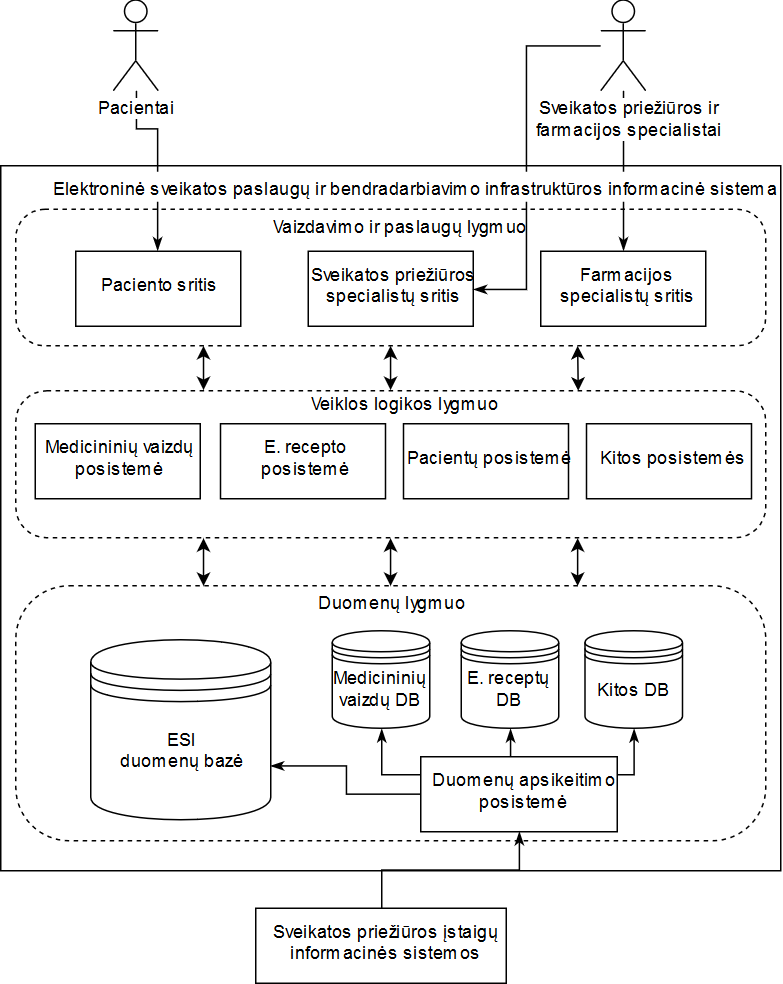
\includegraphics[scale=0.45]{images/ESPBI}
    \caption{Elektroninės sveikatos paslaugų ir bendradarbiavimo infrastruktūros informacinės sistemos achitektūra} 
\end{figure}
% perpiesti, reikia prideti esi posisteme


Pagal parengtos architektūros diagramą matome, kad architektūra yra 3 lygmenų - vaizdavimo ir paslaugų, veiklos logikos ir duomenų lygmens. Išnagrinėkime šiuos tris lygmenis: 

\begin{itemize}
    \item \textbf{Vaizdavimo ir paslaugų lygmuo}. Šį lygmenį sudaro elektroninės sveikatos portalo posistemė. Šio portalo paskirtis - medicininių  paslaugų inicijavimas, šių paslaugų informavimas, jų vykdymo stebėjimas ir suteiktų paslaugų rezultatų pateikimas\cite{Specifikacija}. Šios sistemos naudotojai yra identifikuojami elektroniniu parašu. Prisijungusiam naudotojui yra pateikiamas turinys pagal identifikavimo metu suteiktas prieigas. Elektroninė sveikatos portalo posistemė susideda iš 4 sričių:
    \begin{enumerate}
        \item Viešai prieinama sritis. Šioje elektroninės sveikatos portalo srityje yra pateikiama visiem prieinama informacija. Tam, kad naudotojas pasiektų šią informaciją, jam savo tapatybės identifikuoti nereikia;
        \item Pacientų sritis. Šioje elektroninės sveikatos portalo srityje yra pateikiama paciento gautų paslaugų informacija, rezultatai, išrašytų elektroninių receptų duomenys ir kt;
        \item Sveikatos priežiūros specialistų sritis. Šioje elektroninės sveikatos portalo srityje sveikatos priežiūros specialistai gali pildyti elektroninės sveikatos priežiūros formas, tvarkyti pacientų duomenis, gauti aktualius paciento klinikinius duomenis, medicininius vaizdus, taip pat specialistas, turintis reikiamą prieiga, gali išrašyti pacientui elektroninį receptą, pratęsti jo galiojimo terminą.
        \item Farmacijos specialistų sritis. Ši elektroninės sveikatos portalo sritis yra skirta farmacijos specialistams. Ji leidžia naudotojams  gauti informaciją apie išrašytą elektroninį receptą ir patvirtinti vaistų ar medicininių pagalbos priemonių išdavimo faktą.
    \end{enumerate}
    \item \textbf{Veiklos logikos lygmuo}. Šis lygmuo yra tarpinis tarp vaizdavimo ir duomenų lygmenų.  Veiklos logikos lygmens pagrindinė paskirtis yra priimti sisteminius pranešimus, juos apdoroti, sugeneruoti reikiamą informaciją ir šią informaciją pateikti vaizdavimo ir paslaugų lygmeniui \cite{Specifikacija}. Taip pat šis lygmuo priima duomenis iš elektroninio sveikatos portalo, šiuos duomenis apdoroja ir perduoda į duomenų lygmenį. Apibendrinant šio lygmens paskirtį - tai centrinis funkcionalumų lygmuo, kuris apdoroja ir pateikia reikalingus duomenis apie pacientą, elektroninius receptus, medicininius vaizdus ir kt. Šį lygmenį sudaro 11 posistemių, tačiau pagrindinės yra: 
    \begin{enumerate}
        \item Pacientų posistemė;
        \item Medicininių  vaizdų posistemė;
        \item Elektroninio recepto posistemė;
        \item Duomenų analizės, ataskaitų formavimo ir informavimo posistemė;
        \item Elektroninio sveikatos įrašo posistemė.
    \end{enumerate}
    \item \textbf{Duomenų lygmuo}. Duomenų lygmuo susideda iš 2 komponentų - informacinės struktūros ir duomenų mainų posistemės. Apžvelkime šiuos komponentus:
    \begin{itemize}
        \item Informacinė struktūra. Šis komponentas atsakingas už ESPBI IS informacijos tvarkymą, saugojimą, apdorojimą ir teikimą. Pagrindinis informacinės struktūros komponentas yra ESI duomenų bazė, tačiau informacinė struktūrą sudaro ir daugiau papildomų duomenų bazių \cite{Specifikacija}, iš viso yra 10 duomenų bazių, kurios saugo informaciją apie sveikatos priežiūros paslaugų teikimą. ESI duomenų bazėje saugomi pacientų elektroniniai sveikatos įrašai, kurie yra suvedami paslaugų ir vaizdavimo lygmenyje arba gaunami iš sveikatos priežiūros įstaigų informacinių sistemų. Kiekvienas įrašas yra susiejimas su identifikatoriumi, kuris yra suteikiamas Objektų ID katalogo. Objektų ID katalogas suteiktą identifikatorių susieja su paciento įrašu, specialistu, kuris pateikė paciento įrašą, ir sveikatos priežiūros įstaiga. ESI duomenų bazės tvarkomi dokumentai \cite{Specifikacija}: ypatingieji pacientų duomenys, ESI suformavusių sveikatinimo specialistų duomenys, ESI pateikusių sveikatinimo įstaigų duomenys;
        \item Duomenų mainų posistemė. Šis komponentas atsakingas už duomenų priėmimą bei atidavimą sveikatos priežiūros įstaigų informacinėms sistemoms bei kitoms suinteresuotų trečiųjų šalių informacinėms sistemos. Ši posistemė yra kertinis komponentas, kuris realizuoja techninio interoperabilumo principus elektroninės sveikatos sistemoje \cite{Specifikacija}. Duomenų mainų posistemės pagrindinė paskirtis - valdyti duomenų mainus tarp sveikatos priežiūros įstaigų ir užtikrinti duomenų gavimą bei teikimą tokioms įstaigom kaip SODRA, SVEIDRA, VAPRIS ir kitomis valstybinėms institucijom. Visi duomenų mainai tarp ESPBI IS ir kitų informacinių sistemų vyksta per šią posistemę.
    \end{itemize}
\end{itemize}

\subsubsection{Septinto lygio sveikatos standartas}
Ankstesniuose poskyriuose apžvelgėme Lietuvos sveikatos priežiūros įstaigų naudojamas informacines sistemas, tačiau Lietuva nėra išskirtinė šioje srityje ir kitos Europos sąjungos valstybės taip pat diegia bei naudoja tokio pat pobūdžio informacines sistemas, šių sistemų diegimo bei naudojimo būsena yra aprašyta Europos Komisijos \cite{EuroposKomisija}. Europos parlamento priimtose direktyvose \cite{EuroposParlamentas} yra nurodoma, jog valstybės turi tarpusavyje dalintis pacientų sveikatos įrašais, t.y. pacientui apsilankius svetimos valstybės sveikatos priežiūros įstaigoje, ši įstaiga galėtų gauti paciento duomenis iš jo gimtosios valstybės. Kadangi siekiama pacientų duomenų keitimosi ne tik regioniniu mastu, bet ir tarpvalstybiniu, vadinasi visos tarpusavyje komunikuojančios informacinės sistemos turi vadovautis bendru tarptautiniu standartu, kuris aprašytų pacientų duomenų apsikeitimo procesą. Toks pacientų duomenų apsikeitimo standartas yra Septintojo lygio sveikatos standartas (angl. \textit{Health Level Seven International}) (toliau - HL7). HL7 standartas, kurio pirmoji versija buvo sukurta 1987 metais, yra patvirtintas Amerikos nacionalinio standartų instituto, šis standartas apibrėžia elektroninių sveikatos įrašų paiešką, dalijimąsi, integraciją ir apsikeitimą \cite{HL72009}. HL7 nusako kaip įstaigos keičiasi elektroniniais sveikatos įrašais ir kokiu duomenų formatu šie įrašai yra suformuoti. HL7 yra apibrėžęs 2 duomenų formatus - v2 ir v3, taip pat egzistuoja ir FHIR standartas, kuris apjungia labiausiai pasiteisinusius HL7 v2 ir v3 standartų aspektus. ESPBI IS specifikacijoje \cite{Specifikacija} yra nurodoma, jog duomenų apsikeitimui yra naudojamas HL7 v3 arba FHIR standartai, tačiau naujesnėje literatūroje \cite{Registrucentras} yra nurodomas tik FHIR. FHIR standartas apibrėžia netik duomenų formavimą, bet ir pateikia REST architektūra pagrįstą interfeisą, kuris nurodo
% paaiskint interfeisa ir resta, crud
duomenų operacijoms reikalingus CRUD metodus.


% issiaiskinti del ruklos, kam ji priklauso ( Jei priklauso kazkam is saraso, galim prideti saltini prie hospitalisation.tex)
% neiasku del duomenu baziu, lape raso, kad ji viena yra, o realiai ju daug


\subsection{Stacionariame gydyme pasitaikančių problemų sprendimo būdai}

Su stacionaraus gydymo problemomis, kurios buvo identifikuotos pirmąjame skyriuje, yra susiduriama ne tik Lietuvoje. Jungtinėse Amerikos Valstijose pradėjus sveikatos įstaigose diegti informacines sistemas, atsirado daug problemų, kurios trukdė šių sistemų diegimui bei naudojimui. Viena iš problemų - sveikatos įstaigų darbuotojai nemoka naudotis informacinėmis technologijomis \cite{Jha2009}. Ši problema mažina darbuotojų produktyvumą, nes informacinių sistemų naudojimas užima perdaug laiko. Tam, kad sveikatos priežiūros įstaigų darbuotojai gebėtų efektyviai dirbti su naujausiomis technologijomis, labai svarbus yra jų įtraukimas į diegimo procesą, edukavimas ir kompetentingų žmonių pagalba \cite{Lorenzi2009}. Duomenų įvedimo sunkumai taip pat yra sprendžiami šablonų bei automatinio teksto funkcijomis \cite{Noblin2013}. Darbuotojams yra lengviau pildyti dokumentas pagal pateiktus šablonus bei instrukcijas, o automatinio teksto funkcija paspartina duomenų įvedimą į sistemą. 

Taip pat pirmąjame skyriuje buvo identifikuota medikamentų paruošimo problema. Nors daugiausiai laiko paruošimo procese užima medikamentų rūšiavimas kiekvienam pacientui, tačiau šis etapas yra gyvybiškai svarbus, nes suklydus ir pateikus netinkamą vaistą pacientui, pasekmės gali būti kritinės. Medikamentų adiministravimo problemas siūloma spręsti šiais būdais \cite{Agrawal2009}:
\begin{itemize}
    \item Paskirtų medikamentų informaciją skaitmenitizuoti;
    \item Medikamentus sužymėti brūkšninias kodais (angl. \textit{barcode}), kur brūkšniniame kode būtų laikoma paciento, kuriam paskirtas vaistas, informacija;
    \item Medikamentų užsakymo sistema (angl. \textit{Computerized physician order entry, CPOE}). Ši sistema apjungia sveikatos ir farmacijos įstaigas, padeda atlikti medikamentų užsakymus.
\end{itemize}

Pagal pateiktus problemų sprendimo pavyzdžius matome, kad dauguma jų sprendžia duomenų įvedimo problemą. Ši problema taip pat gali būti sprendžiama artimojo lauko ryšio technologija. Pagrindiniai argumentai, kodėl artimojo lauko ryšio technologija gali padėti spręsti minėtas problemas \cite{forum2}: 
\begin{itemize}
    \item Paprastas paciento duomenų perkėlimas;
    \item Užtikrintumas dėl informacijos tikslumo konkrečiam pacientui;
    \item Paprastas įrenginių prilietimas nereikalauja darbuotojų mokymų;
    \item Lengvas pacientui paskirtų medikamentų identifikavimas.
\end{itemize}

 \newcolumntype{C}[1]{>{\centering\arraybackslash}p{#1}}

\section{Ryšio mažame lauke technologija}

\subsection{Radijo dažnio identifikavimo technologija}
Radijo dažnio identifikavimas (angl. \textit{Radio-frequency identification}) (toliau- RFID) tai viena iš bevielio komunikavimo technologijų, kuri yra paremta elektromagnetinių bangų spektro dažniais, kurie padeda identifikuoti unikalius objektus. Pirmieji RFID panaudojo Britų armijos karininkai Antrajame pasauliniame kare, jie šią technologiją naudojo identifikuoti armijai priklausančius objektus, t.y. lėktuvus, radarus ir kt. \cite{Motlagh2012}. RFID sukuria vienos krypties arba dvikryptį bevielį duomenų srautą. Duomenų perdavime dalyvauja 2 aktoriai - žyma (angl. \textit{tag}), ir skaitytuvas (angl. \textit{reader}) \cite{Igoe2014}. Skaitytuvas inicijuoja komunikavimą sukurdamas elektromagnetinio lauko bangas ir laukia atsakymo iš žymos. Žyma priima skaitytuvo komunikavimo užklausą ir grąžina rezultatą. Žemiau pateiktoje diagramoje (žiūrėti 2 pav.) pavaizduota RFID sistema, šia sistemą bei daugelį kitų RFID sistemų sudaro šie 3 pagrindiniai komponentai \cite{Hunt2006}: 
\begin{enumerate}
    \item \textbf{Žyma}, taip pat dar vadinama - siųstuvu. Žyma yra sudaryta iš semi konduktoriaus mikroschemos, antenos. Taip pat kartais žyma turi vidinį maitinimo šaltinį - bateriją.
    \item \textbf{Skaitytuvas}, jis yra sudarytas iš antenos, radjo bangų dažnių modulio, kuris skirtas siųsti ir gauti signalus iš žymos, ir valdymo modulio.
    \item \textbf{Valdiklis} (angl. \textit{controller}), taip pat dar vadinamas pagrindiniu kompiuteriu (angl. \textit{host}). Dažniausiai tai yra kompiuteris, kuriame yra duomenų bazė ir valdymo programinė įranga.
\end{enumerate}

\begin{figure}[H]
    \centering
    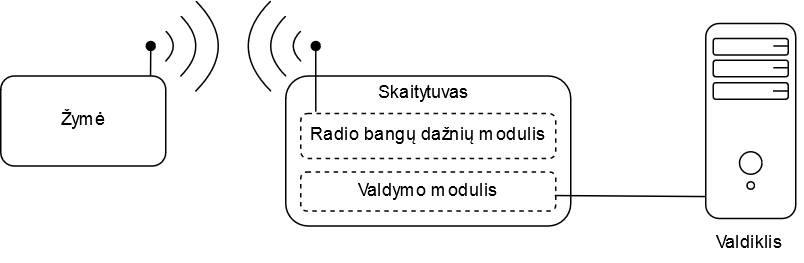
\includegraphics[scale=0.45]{images/RFID}
    \caption{RFID sistemos komponentų diagrama} 
\end{figure}

RFID žymos yra skirstomos į 2 tipus \cite{Igoe2014}:
\begin{enumerate}
    \item Aktyvus komunikavimo tipas. Šiam tipui priklauso tos RFID technologijos, kurių aktoriai turi savo nuosavus energijos šaltinius. Kuomet žyma siunčia rezultatą skaitytuvui, jis naudoja energiją, kuri yra gaunama iš nuosavo maitinimo šaltinio.
    \item Pasyvus komunikavimo tipas. Šiam tipui priklauso tos RFID technologijos, kurių vienas iš aktorių neturi nuosavo energijos šaltinio, t.y. žyma neturi, o siųstuvas turi. Tam, kad žyma išsiųstų rezultatą, ji reikiamą energiją gauna iš iniciatoriaus sukurto magnetinio lauko.
\end{enumerate}
Lentelėje (žiūrėti 2 lentelę) pateikiamas aktyvios ir pasyvius žymos palyginimas.

\begin{table}[!ht]
    \centering
    \renewcommand{\arraystretch}{1,2}
    \begin{tabular}{| p{10em} | p{12em} | p{12em} |}\hline
        \backslashbox[10em]{Ypatybės}{Tipai}
        &\makebox[12em]{Aktyvus}&\makebox[12em]{Pasyvus}\\\hline
        Maitinimo šaltinis & Vidinis & Išorinis\\\hline
        Skaitymo diapazonas & Didelis - iki 100 metrų & Nėra didelis - iki 3 metrų   \\\hline
        Žymos veikimo laikas & Kadangi žyma turi vidinį maitinimo šaltinį, jis nuolatos būna veikimo būsenoje & Žyma pradeda veikti tik tuomet, kai skaitytuvas inicijuoja komunikavimą \\\hline
        Magnetinio lauko stiprumas & Magnetinis laukas nėra stiprus, nes žyma naudoja vidinę energiją tam, kad išsiųstų signalą  & Sukuriamas stiprus magnetinis laukas, nes šio magnetinio lauko dėka, žyma įgyja energijos išsiųsti signalą \\\hline
        Naudojimo terminas & Naudojimo terminas priklauso nuo maitinimo šaltinio galiojimo termino & Naudojimo terminas nėra apibrėžtas \\\hline
        Saugomų duomenų dydis &  Didesnis, dažnu atveju 128 kilobaitai (angl \textit{Kilobyte}) & Mažas, dažniausiai 128 baitai (angl. \textit{Byte})  \\\hline
        Dydis & Dydis priklauso nuo maitinimo šaltinio dydžio & Mažas \\\hline
        Kaina & Brangesnis nei pasyvus & Brangesnis nei aktyvus \\\hline
    \end{tabular}
    \caption{Aktyvios ir pasyvios RFID žymos palyginimas}
\end{table}

RFID technologijos charakteristikos nėra pastovios, šios technologijos savybėm didžiausią įtaką daro parinktas elektromagnetinės bangos dažnis, kuris yra naudojamas komunikavimui tarp skaitytuvo ir žymos, todėl kuriant sistemą, kuri yra paremta RFID technologija, svarbu pasirinkti tinkamą bangos dažnį. RFID technologijos naudojami elektromagnetinių bangų dažniai: kilometrinės bangos žemieji dažniai (toliau - ŽD), dekametrinės bangos aukštieji dažniai  (toliau - AD), decimetrinės bangos ultra aukšti dažniai (toliau - UAD) ir mikrobangų dažniai. Šių dažnių naudojimą RFID sistemose aprašo ISO ir IEC standartai. Elektromagnetinių bangų dažniai daro įtaką šioms RFID savybės \cite{Hunt2006}:
\begin{enumerate}
    \item \textbf{Skaitymo diapazonas}. Žemesnių bangų dažnių RFID skaitymo diapazonas būna mažas. Aukštesnių bangų dažnių RFID skaitymo diapazonas yra didesnis, ypač jeigu naudojamas aktyvus RFID tipas.
    \item \textbf{Aktyvus ir pasyvus RFID}. Istoriškai pasyvus RFID naudodavo ŽD ir AD dažnius, o aktyvus - UAD ir mikrobangų dažnius, tačiau šiuo metu abiejų tipų RFID gali naudotis aukštesnius dažnius, t.y. UAD ir mikrobangų dažnius.
    \item \textbf{Radijo dažnių trukdžiai}. Žemesnių dažnių RFID yra labiau atsparūs interferencijai, nei aukštesnių dažnių RFID.
    \item \textbf{Vandens ir metalo įtaka}. Mikrobangos ir UAD turi didesnę tikimybę būti sugertiems skysčio, todėl šių dažnių RFID nėra tinkamas naudoti šlapiem objektams. Kadangi metalas atspindi elektromagnetines bangas, jos negali prasiskverbti pro jį, tačiau net šalia esantis metalas taip pat gali atspindėti elektromagnetines bangas, todėl tiek aukštesnio dažnio, tiek žemesnio dažnio bangoms metalas daro įtaką. Žemesnio dažnio bangos yra paveikiamos metalo mažiau nei aukštesnio.
\end{enumerate}
Žemiau pavaizduotoje lentelėje (žiūrėti 3 lentelę), pateikiamos RFID tipų naudojami elektromagnetiniai bangų dažniai, jų naudojimą apibrėžiantys standartai \cite{Caglar2016}.

\begin{table}[!ht]
    \centering
    \renewcommand{\arraystretch}{1,5}
    \begin{tabular}{m{9em}m{8em}m{8em}m{8em}} 
        \hline
        Elektromagnetinė banga            & Bangos dažniai    & RFID tipas    &Standartai   \\ 
        \hline
        ŽD                     & 125-134.2 KHz & Pasyvus & ISO 11784 \par ISO/IEC 18000-2A \par ISO/IEC 18000-2B   \\ 
        \hline
        AD                     & 13.56 MHz & Pasyvus  &  ISO 18000-3 \par ISO/IEC 15693 \\ 
        \hline
        \multirow{2}{*}{UAD} & 433 MHz       & Aktyvus   &  ISO 18000-7    \\ 
        \cline{2-4}
                                & 860 ir 915 MHz      &  Pasyvus ir Aktyvus  &  ISO 18000-6A \par ISO 18000-6B \par ISO 18000-6C    \\ 
        \hline
        Mikrobangos                       & 2.45 ir 5.8 GHz         & Pasyvus ir Aktyvus &  ISO 18000-4  \\
        \hline
    \end{tabular}
    \caption{Aktyvaus ir pasyvaus RFID komunikavimo tipų palyginimas}
\end{table}

\subsection{Ryšio mažame lauke}
\subsubsection{Sąvoka}
NFC tai bevielio komunikavimo technologija, šis technologija yra pagrįsta anksčiau minėtos RFID technologijos standartais ir interfeisais, todėl įrenginiai, kurie paremti NFC technologija, gali komunikuoti su dauguma RFID technologijos įrenginių \cite{Motlagh2012}. NFC įrenginiai tarpusavyje komunikuoja 13.56 MHz elektromagnetinių bangų dažniu, duomenų perdavimo greitis svyruoja nuo 106 kilobitu per sekundę iki 424 kilobitų per sekundę \cite{whitepapaer}. Maksimalus veikimo atstumas tarp NFC įrenginių literatūroje minimas ne vienodas, apibendrinus literatūros šaltinius, maksimalus veikimo atstumas yra tarp 4 centimetrų ir 20 centimetrų \cite{whitepapaer} \cite{Motlagh2012} \cite{Leora1980}. Pagrindiniai skirtumai tarp RFID ir NFC technologijų \cite{Leora1980}:
\begin{enumerate}
    \item Komunikavimo atveju, atstumas tarp NFC įrenginių turi būti mažas, o RFID technologijoje naudojant aktyvias žymes, atstumas gali būti žymiai didesnis.
    \item NFC technologijoje naudojamos tik pasyvios žymės, o RFID technologijoje naudojamos tiek aktyvios, tiek pasyvios žymės.
    \item Dėl to, kad komunikavimo atstumas yra mažas, duomenų perdavimas laikomas saugesniu nei RFID.
    \item Dėl to, kad komunikavimo atstumas yra mažas, skaitytuvas komunikuoja su norima žyma, todėl mažėja tikimybė jog skaitytuvo veikimo lauke atsiras keletą žymų.
\end{enumerate}
 

\subsubsection{Duomenų apsikeitimo specifikacija}
NFC duomenų apsikeitimo formatas (angl. \textit{NFC Data Exchange Format}) (toliau - NDEF) tai standartas, kuris nusako duomenų apsikeitimo formatą tarp NFC įrenginio ir NFC žymės arba tarp dviejų NFC įrenginių \cite{Leora1980}. Komunikavimo metu, siunčiama NDEF žinutė, kurią sudaro vienas arba daugiau NDEF įrašų (angl. \textit{records}) (žiūrėti 3 pav.). NDEF įrašą sudaro antraštė (angl. \textit{header}) ir informacija (angl. \textit{payload}), kurios dydis yra iki 2\textsuperscript{32}-1 baitų \cite{NFCForum2006}. Norint talpinti didesnį kiekį duomenų, NDEF įrašai gali būti apjungti. Kadangi NDEF žinutę gali sudaryti daugiau nei vienas įrašas, svarbu indikuoti žinutės rėžius, todėl pirmasis įrašas žinutės eilėje turi žinutės pradžios indikatorių, o paskutinis įrašas - žinutės pabaigos indikatorių.

\begin{figure}[H]
    \centering
    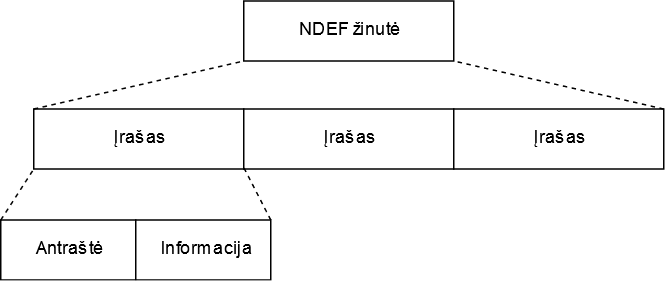
\includegraphics[scale=0.5]{images/NDEF}
    \caption{NDEF žinutės sudedamosios dalys} 
\end{figure}


Žemiau pateiktoje lentelėje (žiūrėti 4 lentelę) yra nurodoma NDEF žinutės įrašą sudarantys laukai. Žinutės įrašą sudaro 12 laukų, iš kuriu 11 sudaro įrašo antraštę, o 1 sudaro informaciją.
Antraštės laukai yra šie \cite{NFCForum2006}: 
\begin{itemize}
    \item \textbf{ŽPR}, Žinutės pradžios indikatorius (angl. \textit{Message begin}), šis laukas yra 1 bito dydžio ir jis nurodo žinutės pradžią.
    \item \textbf{ŽPB}, Žinutės pabaigos indikatorius (angl. \textit{Message end}), šis laukas yra 1 bito dydžio ir jis nurodo žinutės pabaigą.
    \item \textbf{DD}, Duomenų dalis (angl. \textit{Chunk flag}), šis laukas yra 1 bito dydžio ir nurodo ar įrašo informacija yra pilna, ar įraše laikoma informacija yra tik dalis pilnos siunčiamos informacijos.
    \item \textbf{TĮ}, Trumpas įrašas (angl. \textit{Short record}), šis laukas yra 1 bito dydžio, jis nurodo ar informacijos kiekis yra mažesnis nei 2\textsuperscript{8}-1 baitai.
    \item \textbf{IB}, ID būvimas (angl. \textit{ID length present}), šis laukas yra 1 bito dydžio, jis nurodo ar įraše yra saugomas ID.
    \item \textbf{ĮTF}, Įrašo tipo formatas (angl. \textit{Type name format}), šis laukas yra 3 bitų dydžio, jis nurodo kokio formato yra NDEF įrašo tipas. Tipo formatų sąrašas yra pateiktas literatūroje \cite{Leora1980}.
    \item \textbf{Įrašo tipo dydis} (angl. \textit{Type length}), šis laukas yra 1 baito dydžio, jis nurodo koks yra įrašo tipo lauko dydis.
    \item \textbf{ID dydis} (angl. \textit{ID length}), šis laukas yra 1 baito dydžio, jis yra saugomas įraše tuomet, kai IB lauko bitas yra 1. Šis laukas nurodo koks yra ID lauko dydis.
    \item \textbf{Informacijos dydis} (angl \textit{Payload length}), šio lauko dydį nusako TĮ lauko reikšmė. Jeigu TĮ lauko bitas yra 1, tuomet Informacijos dydžio lauko dydis yra 1 baitas. Jeigu TĮ lauko bitas yra 0, tuomet Informacijos dydžio lauko dydis yra 4 baitai.
    \item \textbf{Įrašo tipas} (angl. \textit{Type}), šis lauko dydi nusako Įrašo tipo dydžio laukas. Šis laukas nurodo įrašo informacijos lauko tipą. Įrašo tipas turi būti pateiktas tokiu formatu, kuris yra nurodomas ĮTF lauke.
    \item \textbf{ID}, šio lauko dydį nusako ID dydžio laukas. Šis laukas nurodo įrašo unikalų identifikatorių.
\end{itemize}
Informacijos lauko dydį NDEF įraše nusako antraštės informacijos dydžio laukas. Šiame lauke yra saugoma informacija, kuria yra keičiamasis tarp NFC įrenginių.

\begin{table}[!ht]
    \centering
    \renewcommand{\arraystretch}{1,7}
    \begin{tabular}{C{2em}C{2em}C{2em}C{2em}C{2em}C{2em}C{2em}C{2em}l}
        7                         & 6                        & 5                       & 4                       & 3                       & 2 & 1 & 0                 &                        \\ 
        \hline
        \multicolumn{1}{|c|}{ŽPR} & \multicolumn{1}{c|}{ŽPA} & \multicolumn{1}{c|}{DD} & \multicolumn{1}{c|}{TĮ} & \multicolumn{1}{c|}{IB} & \multicolumn{3}{c|}{ĮTF } & \parbox[t]{2mm}{\multirow{6}{*}{\rotatebox[origin=c]{270}{Antraštė}}}  \\ 
        \cline{1-8}
        \multicolumn{8}{|c|}{Įrašo tipo dydis}                                                                                                                         &                        \\ 
        \cline{1-8}
        \multicolumn{8}{|c|}{Informacijos dydis}                                                                                                                       &                        \\ 
        \cline{1-8}
        \multicolumn{8}{|c|}{ID dydis}                                                                                                                                 &                        \\ 
        \cline{1-8}
        \multicolumn{8}{|c|}{Įrašo tipas}                                                                                                                              &                        \\ 
        \cline{1-8}
        \multicolumn{8}{|c|}{ID}                                                                                                                                       &                        \\ 
        \hline
        \multicolumn{8}{|c|}{}                                                                                                                                         &                        \\
        \multicolumn{8}{|c|}{Informacija}                                                                                                                              &                        \\
        \multicolumn{8}{|c|}{}                                                                                                                                         &                        \\
        \cline{1-8}
    \end{tabular}
    \caption{NDEF žinutės įrašas \cite{NFCForum2006} }
\end{table}

\subsubsection{Darbo rėžimai}
Ryšio mažame lauke technologija turi 3 darbo rėžimus (angl. \textit{operating modes}) - lygiarangių (angl. \textit{peer to peer}), skaitymo ir rašymo (angl. \textit{reader and writer}), kortelės emuliacijos (angl. \textit{emulation}) \cite{whitepaper2}. Kiekvienas darbo rėžimas nurodo kaip ir su kuo NFC įrenginiai komunikuoja. Kiekvienas NFC įrenginys privalo veikti pagal vieną iš trijų darbo rėžimų \cite{Motlagh2012}. Kiekvienas darbo rėžimas turi skirtingas technines infrastruktūras, standartus ir komunikavimo interfeisus, kurie yra aprašyti ISO/IEC 14443, FeliCa, NFCIP-1 \cite{Leora1980}.
Toliau apžvelgsime šiuos 3 darbo rėžimus:
\begin{itemize}
    \item \textbf{Lygiarangiai}. Šiame darbo rėžime du NFC įrenginiai komunikuoja tarpusavyje. Komunikavimas ir informacijos keitimasis tarp įrenginių yra dvikryptis (angl. \textit{bidirectional}). Kadangi įrenginiai yra lygiareikšmiai, todėl jie gali ir inicijuoti bendravimą, ir klausytis. Įrenginiams keičiantis informacija, vienas įrenginys turi siųsti duomenis, o kitas - klausytis ir pradėti siųsti duomenis tuomet, kai pirmasis įrenginys pabaigs siuntimą \cite{Leora1980}. Šio darbo rėžimo specifikuojamas informacijos keitimasis yra laikomas saugiu \cite{Rahul2015}. Literatūroje \cite{Leora1980} yra išskiriamas pagrindinis privalumas - saugus privačių duomenų persiuntimas iš vieno NFC įrenginio į kitą.
    \item \textbf{Skaitymas ir rašymas}. Šiame darbo rėžime komunikacija vyksta tarp NFC įrenginio ir NFC žymės. Šis darbo rėžimas leidžia NFC įrenginiui tiek rašyti, tiek ir skaityti informaciją iš NFC žymos. Rašymo metu įrenginys siunčia duomenis žymai ir jeigu žyma nėra tuščia, jos seni duomenys yra pakeičiami (angl. \textit{overwrite}) naujais \cite{Leora1980}. Komunikacijos metu keičiamasi informacija NDEF žinutės formatu.  Šio darbo rėžimo specifikuojamas informacijos keitimasis nėra laikomas saugiu \cite{Rahul2015}. Literatūroje \cite{Leora1980} yra išskiriami pagrindinis šio darbo rėžimo privalumas - sąlygiškai nesudėtinga šio darbo rėžimo implementacija.
    \item \textbf{Kortelės emuliacija}. Šis darbo rėžimas apibrėžia dviejų NFC įrenginių komunikavimą. Pagrindinis skirtumas tarp lygiarangių darbo rėžimo - kortelės emuliacijoje vienas iš įrenginių emuliuoja informacinę kortelę, o kitas įrenginys gali nuskaityti kortelėje esančius duomenis \cite{Motlagh2012}. Duomenų nuskaitymo metu įrenginys, kuris emuliuoja informacinę kortelę, neskleidžia savo radijo dažnio, o tik klauso aplinkoje esančių dažnių \cite{Leora1980}. Kalbant apie šio darbo rėžimo taikymą, viena iš esminių panaudojimų sričių - atsiskaitymai. Literatūroje \cite{Leora1980} yra išskiriami pagrindinis šio darbo rėžimo privalumas - fizinių objektų eliminavimas, t.y. kreditinės kortelės, bilietai ir kt. gali būti laikomi telefone.
\end{itemize}

\subsubsection{Pritaikymas sveikatos priežiūroje}
Sveikatos priežiūros srityje NFC technologija gali būti taikoma įvairioms užduotims palengvinti. Nyderlanduose ir Prancūzijoje telefonus su įdiegta NFC technologija naudoja virš 50000 slaugytojų \cite{ShyamThangaraju2013}, šios slaugytojos sveikatos paslaugas teikia pacientų namuose. NFC technologija padeda sekti atvykimo ir išvykimo laikus. Administratoriams užtenka šių duomenų paruošti pacientui sąskaitą, todėl slaugytojams nereikia patiems laiko skirti pildant administracinius dokumentus. NFC technologija taip pat naudojama Pakistano sveikatos priežiūroje gydant pneumonijos atvejus \cite{Marcus}. Kaip pabrėžiame literatūroje, Pakistanas yra besivystanti šalis, o NFC technologija sąlygiškai nereikalauja didelių kaštų, todėl NFC technologija gali padėti ir kitom neturtingom valstybėm. Nagrinėjant šiuos du NFC taikymo atvejus ir kitas literatūras susijusias su NFC medicinoje, pastebima jog NFC taikymas nėra paplitęs medicinos srityje, aptikti technologijos panaudojimai yra išimtiniai arba bandomojoje būsenoje ir yra taikomi tik siauroje sveikatos priežiūros srityje. Nepaisant to, jog realių NFC technologijos panaudojimų nebuvo aptikta daug, tačiau literatūrose yra išsamiai nagrinėjamas galimas NFC panaudojimas medicinoje ir siūlomi taikymo būdai bei jų implementacija, todėl tolimesniame nagrinėjime autorius apžvelgia literatūrose siūlomus NFC panaudojimo būdus. Literatūroje išskiriami 2 pagrindiniai NFC technologijos taikymo klasifikatoriai \cite{Gautam}:
\begin{itemize}
    \item \textbf{Išorinis taikymas}. Šiame klasifikatoriuje yra visi NFC panaudojimo atvejai, kurie skirti:
        \begin{itemize}
            \item Tvarkyti paciento elektroninį sveikatos įrašą;  
            \item Sekti medicininių įrankių inventorizaciją;
            \item Valdyti medikamentų išdavimą;
        \end{itemize}
    \item \textbf{Vidinis taikymas}. Šiame klasifikatoriuje yra visi NFC panaudojimo atvejai, kurie skirti sekti paciento simptomus, organizmo būseną.
\end{itemize}
 
Dalis literatūrose aprašomų NFC panaudojimo atvejų yra skirti stebėti pacientų būklę \cite{Strommer2006} \cite{Gautam} \cite{Zhang2011}. Pacientų būklę sekantys įrenginiai, tokie kaip - gliukozės kiekio kraujyje matuoklis, širdies pulso ir spaudimo matuoklis ir kt., jau egzistuoja rinkoje ir naudojami medicinoje daug metų. Jeigu minėtų įrenginių rodmenys privalo būti sekami ir saugomi, vadinasi gautus duomenis reikia kažkur išsaugoti, šis procesas yra atliekamas arba rankinių būdų, t.y. sveikatos priežiūros darbuotojai perrašo gautus duomenis į saugojimo aplinkas, arba įrenginiai veikai kartu su servisais, kurie turi prieiga prie duomenų bazės, ir duomenų saugojimas vyksta be darbuotojų įsikišimo. Literatūroje \cite{Strommer2006} identifikuojama, jog tokie įrenginiai dažniausiai būna prijungti prie kompiuterio laidais, o toks komunikavimo būdas tarp kompiuterio ir medicinos įrenginių yra nepatogus, nes kiekvienas įrenginys turi laidinę išvestį, o didinat įrenginių skaičių didėja laidų kiekis, todėl NFC technologija sprendžią šią problemą pašalindama laidinį komunikavimą \cite{Strommer2006}. Įrenginių rodmenų saugojimo eiga yra aprašyta literatūroje \cite{Zhang2011}.

Jungtinėse Amerikos Valstijose per metus apie 1500 medicininių objektų yra per klaidą paliekami pacientų kūnuose operacijų metu \cite{RamaKrishnaPrasad}. Šiai problemai spręsti yra naudojama NFC technologija. Medicininiai objektai, kurie neturi likti pacientų kūne, yra sužymimo NFC žymomis, tai padeda medikams atsekti ar pacientų kūnuose per klaidą liko medicininiai objektai. Šis pavyzdys yra vienas iš daugelio literatūrose \cite{Ajami2014} \cite{Puma2012} \cite{Azlina2013} pateikiamų NFC ir RFID technologijų taikymo būdų, skirtų medicininių įrenginių, objektų inventorizacijai. Jungtinėse Amerikos Valstijose viena iš sveikatos priežiūros įstaigų problemų - medicininės įrangos ar įrankių vagystės, šioje valstybėje per metus prarandama beveik 4 milijardus JAV dolerių vertų medicininių įrankių ir įrangos \cite{RamaKrishnaPrasad}, šioje literatūroje teigiama jog RFID technologijos gali padėti spręsti šią problemą.

Taip pat dalis literatūrose aprašomų NFC taikymo būdų yra skirti palengvinti pacientų elektroninio sveikatos įrašo valdymą, padidinti pacientų duomenų valdymo efektyvumą \cite{Gautam} \cite{RamaKrishnaPrasad} \cite{Fontecha2011} \cite{Davcev2015}. Visose minėtose literatūrose yra siūloma priskirti pacientui NFC žymą pažymint paciento lovą, apyrankę ar palatą. Priskirtą žymą yra siūloma užpildyti paciento duomenimis tam, kad įstaigų darbuotojams prireikus šių duomenų, juos gauti būtų patogu ir greita. Nors minėtas pasiūlymas didina duomenų gavimo greitį, tačiau svarbu atkreipti dėmesį į saugumo spragas, nes žymes, kurios turi svarbius paciento duomenis, gali būti nuskaitytos ne tik įstaigų darbuotojų ir taip pacientų duomenys gali būti nutekinti. Apie minėta saugumo spragą užsimenama tik vienoje literatūroje \cite{RamaKrishnaPrasad}.

Aptartuose NFC technologijos panaudos atvejus sveikatos priežiūros srityje, matome, jog ši technologija gali padėti didinti šios srities procesų efektyvumą.


% \subsection{NFC techologijos dabartis ateitis} ???
% \subsection{NFC technologijos palyginimas} ???




\section{Sistemos projektavimas}


\subsection{Reikalavimų surinkimas}
Programų sistemų architektūros yra reikalingos kuriant sistemas, kurios įgyvendina keliamus reikalavimus \cite{Bass2013}, o kadangi šio baigiamojo darbo tikslas - pasiūlyti architektūrą, labai svarbu apsibrėžti keliamus sistemos reikalavimus. Šiame poskyryje bus pateikiami funkciniai ir nefunkciniai sistemos reikalavimai. Tam, kad apsibrėžti svarbius reikalavimus, svarbu analizuoti dalykinę sritį, esamą situaciją. Surinkdamas reikalavimus, autorius remiasi skyriuje identifikuotomis dalykinės srities problemomis, antrajame skyriuje analizuotomis informacinėmis sistemomis ir nagrinėta literatūra.
\subsubsection{Funkciniai reikalavimai}

Funkciniai reikalavimai yra surinkti remiantis dalykinės srities analize ir identifikuotomis stacionaraus gydymo problemomis.

\begin{table}[!ht]
    \centering
    \renewcommand{\arraystretch}{1.2}
    \renewcommand\thetable{5}

    \begin{tabular}{|m{3em}|m{17em}|m{17em}|}
    \hline 
    \rowcolor[HTML]{EFEFEF} 
    Reik. Nr. & Reikalavimas & Aprašymas \\ \hline
    FR.1  &  Duomenų įvedimas galimas ALR technologijos pagalba  & Reikalavimas kyla iš stacionaraus gydymo problemų sprendimo būdų  (žiūrėti 2.3. poskyrį)    \\ \hline
    FR.2  &  Sistemos vidiniai naudotojai yra autorizuojami  &  Visi darbuotojai, kurie yra susiję su stacionariu gydymu,  yra identifikuojami, todėl svarbu, kad sistema autorizuotų naudotojus       \\ \hline
    FR.3  &  Sveikatos įstaigos darbuotojas, kuris turi atitinkamą rolę, gali sukurti gydymo planą  &   Reikalavimas kyla iš dalykinės srities (žiūrėti 1. skyrių)       \\ \hline
    FR.4  &  Pacientai yra identifikuojami ESPBI IS pagalba  &  Visų Lietuvos pacientų duomenys yra laikomi ESPBI IS, todėl sistema turi sugebėti komunikuoti su šia sistema      \\ \hline
    FR.5  &  Suteikta sveikatos paslauga yra identifikuojama  &   Reikalavimas kyla iš dalykinės srities (žiūrėti 1. skyrių)      \\ \hline
    FR.6  &  Kiekviena sąveika tarp slaugytojo ir paciento, kuri yra nurodyta gydymo plane, yra fiksuojama ir saugoma  &   Reikalavimas kyla iš dalykinės srities (žiūrėti 1. skyrių)       \\ \hline
    FR.7  &  Sveikatos įstaigos darbuotojas, kuris suteikė bet kokią sveikatos paslaugą, yra identifikuojamas  &   Reikalavimas kyla iš dalykinės srities (žiūrėti 1. skyrių)        \\ \hline
    
    \end{tabular}
    \caption{Projektuojamos sistemos funkciniai reikalavimai} 
\end{table}

\begin{table}[!ht]
    \centering
    \renewcommand{\arraystretch}{1.2}
    \renewcommand\thetable{5}
    \begin{tabular}{|m{3em}|m{17em}|m{17em}|}
    \hline 
    \rowcolor[HTML]{EFEFEF} 
    Reik. Nr. & Reikalavimas & Aprašymas \\ \hline
    FR.8  &  Medikamentų, kurie yra suteikiami pacientui, tinkamumo verifikavimas   &  Patikrinimas ar suteikiamas medikamentas yra nurodytas gydymo plane ir neįvyko klaida. Reikalavimas kyla iš stacionaraus gydymo problemų sprendimo būdų  (žiūrėti 2.3. poskyrį)       \\ \hline
    FR.9  &  Paciento būklės duomenys, gauti suteikiant sveikatos paslaugą, yra fiksuojami ir saugomi  &    Reikalavimas kyla iš dalykinės srities (žiūrėti 1. skyrių)       \\ \hline
    FR.10  &  Formos, reikalingos stacionariame gydyme, yra pildomos sistemoje automatiškai, užpildant formą duomenimis, kurie buvo fiksuoti gydymo metu;  &   Reikalavimas kyla iš stacionaraus gydymo problemų sprendimo būdų  (žiūrėti 2.3. poskyrį)       \\ \hline
    FR.11  &  Medicininių įrašų valdymo veiksmus gali atlikti tik tie darbuotojai, kurie turi valdymo veiksmams reikalingas roles  &  
    Slaugytojai gali redaguoti tik su jais susijusius įvestus duomenis, tačiau gydytojai gali redaguoti visus įvestus duomenis. Reikalavimas kyla iš dalykinės srities (žiūrėti 1. skyrių)       \\ \hline
    FR.12  &  Duomenų mainuose su centralizuota duomenų baze yra naudojamas HL7 formatas  &   Reikalavimas kyla iš sveikatos įstaigų informacinių sistemų analizavimo (žiūrėti 2.2.3 poskyrį)       \\ \hline
    \end{tabular}
    \caption{Projektuojamos sistemos funkciniai reikalavimai} 

\end{table}


\subsubsection{Nefunkciniai reikalavimai}
Nefunkciniai reikalavimai yra surinkti remiantis dabartinių sveikatos įstaigų naudojamomis informacinėmis sistemomis ir literatūra, kuri nagrinėja ALR panaudojimą sveikatos priežiūroje. Surinkti nefunkciniai reikalavimai apima šiuos reikalavimas:
\begin{itemize}
    \item Saugumo ir slaptumo reikalavimai;
    \item Ergonominiai reikalavimai;
    \item Prieinamumo ir patikimumo reikalavimai;
    \item Plečiamumo reikalavimai.
\end{itemize}

\begin{table}[!ht]
    \centering
    \renewcommand{\arraystretch}{1.2}
    \renewcommand\thetable{6}
    \begin{tabular}{|m{3em}|m{17em}|m{17em}|}
    \hline 
    \rowcolor[HTML]{EFEFEF} 
    Reik. Nr. & Reikalavimas & Aprašymas \\ \hline

    NFR.1  &  Vartotojo sąsaja turi būti pritaikyta neįgaliesiems pagal „Web Content Accessibility Guidelines 1.0“ pasiūlymus  &  Reikalavimas kyla remiantis ESPBI IS nagrinėjimu(žiūrėti 2.2. poskyrį)       \\ \hline
    NFR.2  &  Vartotojo sąsaja turi būti daugiakalbė &  Reikalavimas remiasi nagrinėtomis Lietuvos sveikatos įstaigų informacinėmis sistemomis (žiūrėti 2.1. poskyrį)       \\ \hline


    \end{tabular}
    \caption{Projektuojamos sistemos nefunkciniai reikalavimai} 

\end{table}

\begin{table}[!ht]
    \centering
    \renewcommand{\arraystretch}{1.2}
    \renewcommand\thetable{6}

    \begin{tabular}{|m{3em}|m{17em}|m{17em}|}
    \hline 
    \rowcolor[HTML]{EFEFEF} 
    Reik. Nr. & Reikalavimas & Aprašymas \\ \hline
    NFR.3  & Klaidų pranešimai formuojami taip, kad vartotojui būtų aiškų kokių veiksmų imtis  &   Reikalavimas remiasi nagrinėtomis Lietuvos sveikatos įstaigų informacinėmis sistemomis (žiūrėti 2.1. poskyrį)       \\ \hline
    NFR.4  &  Sistemos integracija su skirtingų sveikatos įstaigų informacinėmis sistemomis neturi būti sudėtinga  &   Reikalavimas remiasi nagrinėtomis Lietuvos sveikatos įstaigų informacinėmis sistemomis (žiūrėti 2.1. poskyrį)       \\ \hline
    NFR.5  &  Sistemos našumo plėtimas, gerinant ar didinant techninius išteklius, neturi būti sudėtingas, našumo plėtimas neturi reikalauti programos kodo keitimo  &   Reikalavimas kyla remiantis ESPBI IS nagrinėjimu (žiūrėti 2.2. poskyrį)       \\ \hline
    NFR.6  &   Sistema turi veikti pagal principą „24 valandos per dieną, 7 dienos per savaitę, 365 dienos per metus“  &  Reikalavimas kyla remiantis ESPBI IS nagrinėjimu (žiūrėti 2.2. poskyrį)       \\ \hline
    NFR.7  &  Sistemos, kuri susidūrė su sutrikimais, reikalaujančiais sistemos paleidimo iš naujo, prastovos laikas negali viršyti 3 valandų  &   Reikalavimas kyla remiantis ESPBI IS nagrinėjimu (žiūrėti 2.2. poskyrį)       \\ \hline
    NFR.8  &  Sistemos, kuri susidūrė su sutrikimais, reikalaujančiais sistemos diegimo iš naujo, prastovos laikas negali viršyti 6 valandų  &   Reikalavimas kyla remiantis ESPBI IS nagrinėjimu (žiūrėti 2.2. poskyrį)       \\ \hline
    NFR.9  &  Identifikavimo informacija turi būti šifruojama  &   Reikalavimas remiasi nagrinėtomis Lietuvos sveikatos įstaigų informacinėmis sistemomis (žiūrėti 2.1. poskyrį)       \\ \hline
    \end{tabular}
    \caption{Projektuojamos sistemos nefunkciniai reikalavimai} 

\end{table}

\subsection{Projektuojamos sistemos architektūra}
Programų sistemos architektūra, tai struktūrų rinkinys, kuris apima sistemos elementus, jų tarpusavio ryšius ir savybes \cite{Bass2013}. Kadangi visos programų sistemos turi architektūras \cite{Bass2013}, šiame poskyryje apžvelgiama projektuojamos sistemos architektūra.

\subsubsection{Projektuojamos sistemos priklausomybė nuo dabartinių sistemų}
Lietuvos sveikatos priežiūros įstaigas galima suskirstyti į dvi grupes - tiesiogiai naudojančios ESPBI IS ir netiesiogiai naudojančios ESPBI IS. Tiesiogiai ESPBI IS naudojančios įstaigos savo informacinės sistemos neturi, o netiesiogiai naudojančios įstaigos naudoja savo vidinę informacinę sistemą. Visos vidinės sistemos turi pacientų identifikavimo, duomenų saugojimo ir valdymo modulius. Šiame poskyryje nagrinėjama projektuojamos sistemos integracija su dabartinėmis sveikatos įstaigų vidinėmis informacinėmis sistemomis.

\textbf{Sistema yra posistemė dabartinių sistemų}. Antrajame skyriuje nagrinėtos sveikatos įstaigų informacinės sistemos yra sudarytos iš posistemių. Posistemes sudaro funkcionalumo aibės, kurios atitinka dalykinės srities poreikius, t.y. radiologijos reikmėms yra skirta radiologijos posistemė, laboratorijos reikmėms - laboratorijos posistemė, administravimo reikmėms - administravimo posistemė ir t.t. Kuriant sistemą, kaip dabartinės sistemos posistemę, reikėtų papildyti esamą vartotojo sąsaja su naujos posistemės teikiamais funkcionalumais, atlikti pakeitimus administravimo posistemėje. Taip pat gali būti neišvengiami kitų posistemių koregavimai. Jeigu projektuojama sistema būtų integruojama į daugiau sveikatos įstaigų, naująją sistemą reikėtų pritaikyti skirtingose informacinėse sistemos, nes skirtingos įstaigos turi skirtingas sistemas. Šis sistemos pasirinkimas reikštų, kad projektuojamą sistema galėtų naudoti tik savo  informacines sistemas turinčios sveikatos įstaigos, tačiau kuriant tokią sistemą, didelė dalis reikalavimų, kilusių iš dalykinės srities, būtų įgyvendinti įstaigos informacinės sistemos, nereikėtų kurti modulių, kurių pagalba komunikuojama su ESPBI IS.

\textbf{Sistema nėra priklausoma nuo dabartinių sistemų}. Kadangi ne visos sveikatos įstaigos turi savo vidines informacines sistemas, viena iš alternatyvų - kurti sistemą, kuri visus keliamus reikalavimus įgyvendintų pati ir nebūtų priklausoma nuo dabartinių įstaigų vidinių sistemų. Kadangi visos sveikatos įstaigos yra priklausomos nuo ESPBI IS suteikiamų duomenų, todėl visos sistemos, manipuliuojančios šiais duomenimis, privalo komunikuoti su ESPBI IS, vadinasi, kuriama sistema turėtų pati valdyti duomenų mainus. Projektuojamos sistemos funkcionalumo poaibis sutaptų su dabartinių sistemų funkcionalumų poaibiais. Tokią sistemą galima būtų diegti tiek į įstaigas, kurios neturi vidinių informacinių sistemų, tiek į tas, kurios turi. Diegiant sistemą į įstaigas, kurios turi vidines informacines sistemas, nereikėtų papildomų kaštų vidinių sistemų koregavimui ir jų pritaikymui projektuojamai sistemai, todėl diegimas į visas įstaigas būtų vienodas. Jeigu būtų pasirinkta ši sistema, atsirastų daug funkcionalumo ir duomenų dubliavimo, tačiau ši problema kiltų tik tose įstaigose, kurios turi vidines sistemas. Taip pat šios sistemos kūrimo kaštai būtų didesni nei pirmojo pasiūlymo, nes reikėtų implementuoti daugiau funkcionalumų ir atsirastų duomenų bazė, kurioje būtų laikomi sistemai reikalingi duomenys, kurie nėra gaunami iš ESPBI IS.

\textbf{Sistema yra dalinai priklausoma nuo dabartinių sistemų}. Vienas iš pasirinkimų galėtų būti dalinis sistemos priklausomumas nuo dabartinių sistemų. Projektuojama sistema pati nedalyvautų duomenų mainuose su ESPBI IS, tačiau turėtų tarpinį sluoksnį, kuris bendrautų su dabartinių sistemų duomenų mainų sluoksniu. Šis lygmuo pasirūpintų, kad sistema gautų norimus duomenis. Likusi sistemos dalis būtų savarankiška ir nepriklausytų nuo kitų sistemų, t.y. suprogramavus vartotojo sąsają bei įgyvendinus visus funkcionalumus, jų pritaikyti dabartinėms sistemoms nereikėtų. Diegiant sistemą į skirtingas sveikatos priežiūros įstaigas, kurios turi vidines sistemas, reikėtų koreguoti tik sistemų sąlyčio taškus, t.y. projektuojamos sistemos tarpinis sluoksnis ir vidinių sistemų duomenų mainų sluoksniai. Jeigu sveikatos įstaiga neturi vidinės sistemos, papildomai reikėtų suprojektuoti ir įdiegti duomenų ir duomenų mainų sistemą. Jeigu būtų pasirinkta ši sistema, būtų išvengiamas funkcionalumų ir duomenų dubliavimas, tačiau kiekvienai vidinei sistemai reikėtų pritaikyti naująją sistemą, o jeigu nėra vidinės sistemos, reikėtų papildomų kaštų trūkstamoms sistemos dalims suprojektuoti ir sudiegti.

Norint projektuoti sistemą, kuri būtų posistemė dabartinių sistemų, reikėtų išsikelti prielaidą, kad sistema yra diegiama tik tuose sveikatos įstaigose, kuriose veikia vidinės informacinės sistemos. Pasirinkus šį pasiūlymą ne tik sumažėtų sveikatos įstaigų, kuriose galima pritaikyti sistemą, skaičius, bet ir kiekvienos įstaigos vidinei sistemai reikėtų pakeitimų. Norint išvengti minėtų problemų, galima kurti sistemą, kuri nėra priklausoma nuo dabartinių sistemų, tačiau susidurtume su naujomis problemomis - funkcionalumo bei duomenų dubliavimo ir didesnių sistemos kūrimo kaštų. Paskutinis pasiūlymas, kur sistema yra dalinai priklausoma nuo dabartinių sistemų, spręstų visas minėtas problemas, išskyrus vidinių sistemų pakeitimus, todėl šis pasirinkimas yra tinkamiausias.
% \subsubsection{Prielaidos}
% \textbf{IT} infrastruktūra. Lieuvos sveikatos priežiūros įstaigas galima suskirstyti į dvi grupes - tiesiogiai naudojančios ESPBI IS ir netiesiogiai naudojančios ESPBI IS. Tiesiogiai ESPBI IS naudojančios įstaigos savo informacinės sistemos neturi, o netiesiogiai naudojančios įstaigos naudoja savo vidinę informacinę sistemą. Visos vidinės sistemas turi pacient identifikavimo, duomenų saugojimo ir valdymo modulius.

% zmones turi bazines kompiuterio naudojimo zinias

\subsubsection{Architektūros stilius}
Šiame poskyryje apžvelgiami galimi būsimos sistemos architektūros stiliai. Taip pat pasirenkamas tinkamiausias stilius iš apžvelgtųjų. 

\textbf{Komponentais pagrįstas architektūros stilius}. Komponentinis architektūros stilius yra pagrįstas sistemos išskaidymu į smulkesnius funkcinius ir loginius elementus, kurie yra vadinami komponentais. Jungiant komponentus tarpusavyje, gaunama pilna sistema. Kiekvienas komponentas turi apsibrėžęs komunikavimo sąsają (angl. \textit{interface}), kurioje nurodomi kokie komponento įgyvendinti metodai yra pasiekiami kitiems komponentams. Vienas iš pagrindinių šios architektūros bruožų - komponentų perpanaudojimas. Kadangi kiti komponentai komunikuoja tik per komponento sąsają, komponentą yra lengva pakeisti kitu komponentu, turinčiu tokią pačia sąsają. Kuriant sistemą, kurios architektūros stilius būtų komponentinis, susidurtume su dideliais sistemos kaštais \cite{Component}, nes perpanaudojamų komponentų kūrimas pareikalautų daug laiko ir pastangų, o tai reikštų kaštų didėjimą;

\textbf{Daugiasluoksnės architektūros stilius}. Šis architektūros stilius yra pagrįstas sistemos skaidymu į loginius sluoksnius ir fizinius lygmenis. Kiekvienas sluoksnis turi savo rolę ir atsakomybę (pvz.: verslo logikos, vaizdavimo ir t.t.), todėl kiekvienas sluoksnis atlieka veiksmus susijusius tik su jo logika, o kitų sluoksnių logika jam nėra aktuali. Fiziniai lygmenys yra atskirti fiziškai, t.y. kiekvienas fizinis lygmuo veikia ant skirtingų kompiuterių, tačiau vienam fiziniame lygmenyje gali būti keletas loginių sluoksnių. Tokia architektūra leidžia sistemai būti tiek vertikaliai, tiek horizontaliai plečiamai \cite{By}. Taip pat ši architektūra yra paprastesnė nei komponentinė, todėl jos kūrimo kaštai yra mažesni, tačiau augant sluoksnių skaičiui, sistemos sudėtingumas ir kūrimo kaina didėja.

\textbf{Netaikyti architektūros stilių}. Taip pat vienas iš variantų, sistemos architektūros stiliaus pasirinkime, yra visai netaikyti architektūros stilių. Toks pasirinkimas leistų  greitai sukurti sistemą, nes kūrimo metu nereikėtų laikytis taisyklių ir nevaržytų apribojimai, kurie kyla iš architektūrų stilių. Kadangi šis pasirinkimas leistų sistemą greitai sukurti, vadinasi jos kūrimo kaštai nebūtų dideli. Jeigu nebūtų taikomas joks architektūros stilius, vadinasi sistema būtų labai sunkiai plečiama, o auganti techninė skola (angl. \textit{techincal debt}) didintų sistemos palaikymo kaštus, todėl sistemos bendra kūrimo ir palaikymo kaina būtų didelė. Ši alternatyva nėra laikoma geros architektūros praktika \cite{Bass2013}.

Renkantis sistemos architektūros stilių, svarbu atkreipti dėmesį į sistemai keliamus reikalavimus, taip pat atkreipti dėmesį į sistemos kaštus. Jeigu pasirinktume netaikyti jokio stiliaus, vadinasi sistema sukurti nebus brangu, tačiau jos palaikymo kaštai bus dideli. Jeigu pasirinktume komponentinį architektūros stilių, sistemos architektūra būtų sudėtinga, o sistemos kūrimo kaštai dideli. Daugiasluoksnės architektūros stilius leistų sistemai būti plečiamai bei sistemos kaštai būtų mažesni nei komponentinės, todėl šis stilius yra tinkamiausias kuriant siūlomą sistemą.


\subsubsection{ALR skaitytuvas ir sistemos vartotojo sąsaja}

Teigiama, jog nuo 2015 metų, 50\% rinkoje naudojamų mobiliųjų telefonų turi įdiegtą ALR technologiją \cite{forum2}. Taip pat dauguma literatūrų, kurios analizuoja sveikatos priežiūrą ir ALR technologiją, renkasi mobilųjį telefoną kaip ALR skaitytuvą \cite{Azlina2013} \cite{Strommer2006} \cite{Puma2012} \cite{Marcus} \cite{Gautam}. Malaizijoje atlikta apklausa rodo, kad didžioji dalis sveikatos priežiūros įstaigų darbuotojų rinktųsi naudoti mobiliuosius telefonus kaip ALR skaitytuvus \cite{Azlina2013}. Kadangi dauguma mobiliųjų telefonų turi įdiegtą ALR technologiją ir literatūrose siūloma juos panaudoti ALR įgalintose sistemose, mobilusis telefonas būtų tinkamas projektuojamos sistemos ALR skaitytuvas. Kadangi duomenis, kurie yra įvesti į sistemą, galima matyti ir koreguoti, sistemos naudojimui reikalinga vartotojo sąsaja. Toliau šiame poskyryje apžvelgiami vartotojo sąsajos dislokavimo variantai.

\textbf{Vartotojo sąsaja ALR skaitytuve}. Kliento sluoksnis ir ALR valdiklių sluoksnis gali būti viename lygmenyje, t.y. tiek vartotojo sąsaja, tiek ALR skaitytuvas gali būti viename įrenginyje. Nuskaičius ALR žymą, naudotojas iš karto gali matyti įvestus duomenis, juos redaguoti, išsaugoti. Naudotojui tai būtų patogu, nes jis visus sistemos funkcionalumus gali pasiekti viename įrenginyje. Pasirinkus šį sprendimą, jeigu ALR skaitytuvas būtų nedidelio dydžio, naudotojui gali kilti nepatogumų pildant, redaguojant ir skaitant formose pateiktus duomenis.

\textbf{Vartotojo sąsaja kompiuterio programinėje įrangoje}. Taip pat vartotojo sąsaja gali būti kaip kompiuterio programinė įranga. Nuskaičius ALR žymą, nuskaityti duomenys atsirastų kompiuterio programinėje įrangoje, kur vartotojas galėtų duomenis redaguoti, peržiūrėti ir išsaugoti. Jeigu būtų pasirinktas šis variantas, kiekviename kompiuteryje reikėtų įdiegti šią programinę įrangą. Taip pat, programinę įrangą reikėtų kurti skirtingoms kompiuterių operacinėms sistemoms, o tai padidintų kuriamos sistemos kaštus. Kadangi ALR žymės būtų nuskaitomos su vienu įrenginiu, o duomenų redagavimas ir vaizdavimas atliekamas su kitu, naudotojui gali kilti nepatogumų vaikštant nuo paciento iki artimiausio kompiuterio. Tačiau tuo atveju, kuomet duomenų redagavimui interakcija su paciento ALR žyme nėra reikalinga, naudotojui būtų patogiau redaguoti duomenis naudojantis kompiuteriu, o ne mobiliuoju telefonu. 

\textbf{Vartotojo sąsaja interneto naršyklėje}. Kadangi šiuo metu interneto naršyklė yra įdiegta tiek į stacionarius ir nešiojamus kompiuterius, tiek į mobiliuosius telefonus bei planšetinius kompiuterius, projektuojamos sistemos vartotojo sąsaja galėtų būti pasiekiama per interneto naršyklę. Šis sprendimas leistų išvengti skirtingų operacinių sistemų keliamų sunkumų. Jeigu vartotojo sąsaja būtų pritaikyta mažiems įrenginiams (angl. \textit{responsive}), sistema būtų patogu naudotis neatsižvelgiant į įrenginio dydį. Pasirinkus šį variantą, naudotojas galėtų pasirinkti duomenų redagavimo operacijoms naudoti ALR skaitytuvą, ar kitą įrenginį. 


Visų nagrinėtų informacinių sistemų (žiūrėti 2. skyrių), kurios yra naudojamos sveikatos priežiūros įstaigų darbuotojų, vartotojo sąsajos yra pasiekiamos interneto naršyklėje, todėl tikėtina, kad naudotojai greičiau išmoktų naudotis sistema, jeigu projektuojamos sistemos vartotojo sąsaja būtų pasiekiama interneto naršyklėje. Kadangi siūloma naudoti mobilųjį telefoną kaip ARL skaitytuvą, naudotojai galėtų pasirinkti ar duomenis koreguoti mobiliajame telefone, ar kompiuteryje. Dėl išvardintų priežasčių, vartotojo sąsaja interneto naršyklėje yra tinkamiausias variantas.

\subsubsection{Medikamentų išdavimas}
Medikamentų išdavimo procedūra yra viena iš pagrindinių stacionaraus gydymo paslaugų (žiūrėti 1. skyrių). Šiame poskyryje pateikiama medikamentų išdavimo sekų diagrama (žiūrėti 4 pav.). Šios procedūros tikslas - išduoti medikamentą pacientui ir užfiksuoti šį faktą medicininiu įrašu. Šios diagramos pirminis agentas - sistemos naudotojas, t.y. slaugos darbuotojas arba gydytojas. Šią sekų diagramą sudaro 25 žingsniai, tačiau jeigu išduodamas netinkamas medikamentas, procedūrą sudaro 13 žingsnių, o jeigu naudotojas nenori atšaukti medikamento išdavimo, procedūrą sudaro 19 žingsnių.

\begin{figure}[H]
    \centering
    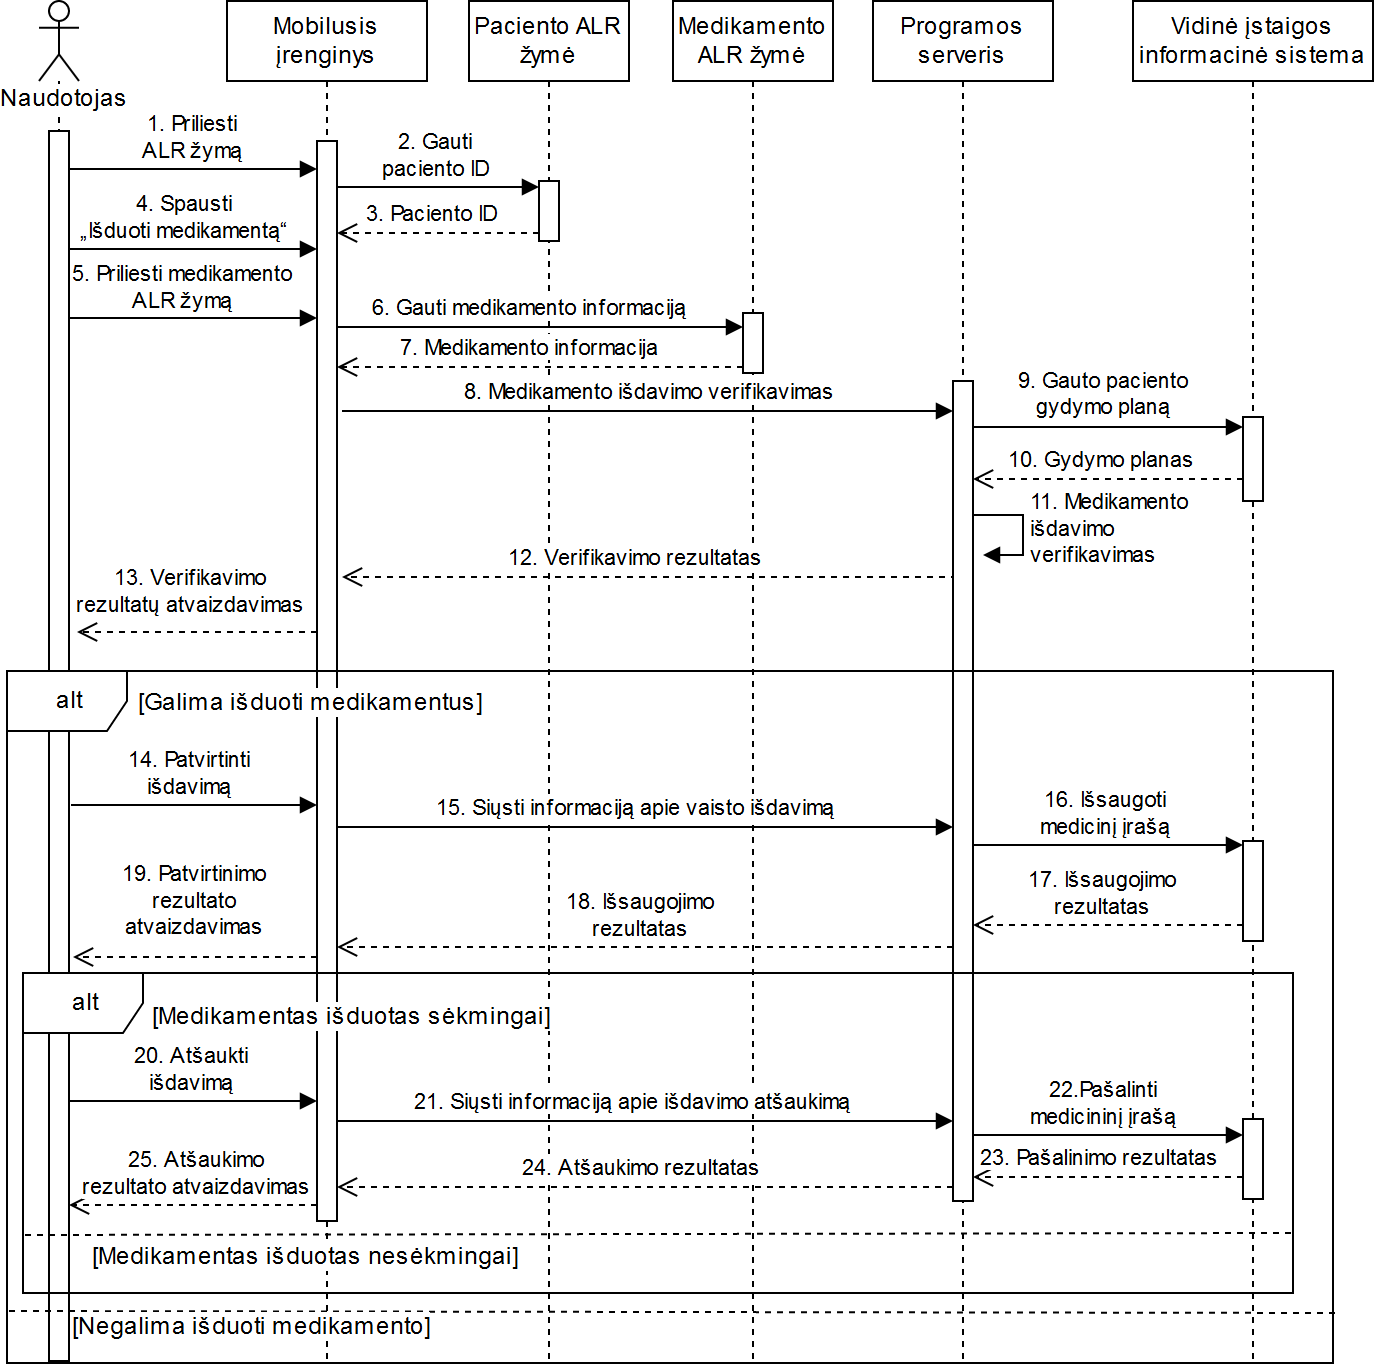
\includegraphics[scale=0.27]{images/israsytiVaistai}
    \caption{Medikamentų išdavimo sekų diagrama} 
\end{figure}

Medikamentų išdavimo procedūrą gali sudaryti mažesnis žingsnių kiekis, todėl toliau pateikiamos šios procedūros žingsnių alternatyvos


\textbf{Atsisakyti „Išduoti medikamentą“ ir „Patvirtinti“ mygtukų}. Atsisakius šių dviejų mygtukų paspaudimo, naudotojui vietoj 5 žingsnių, šiai procedūrai atlikti užtektų 3 žingsnių. Tačiau sumažėjus naudotojo žingsnių kiekiui, naudotojui gali tapti neaišku kokį sekantį žingsnį jis turi atlikti, nes nuskaičius paciento ALR žymą, intuityviai reikėtų žinoti, kad iš karto reikia priliesti ir medikamento ALR žymą. Jeigu šių mygtukų nebūtų, naudotojui gali kilti keblumų kuomet nuskaitoma keleto pacientų ALR žymos ir tuomet nuskaitoma medikamento ALR žyma, šio scenarijaus atveju, gali kilti neaiškumų dėl konkretaus paciento, kuriam turėjo būti išduotas medikamentas.

\textbf{Paciento gydymo plano informaciją laikyti ALR žymoje}. ALR žymoje laikant visą reikiamą informaciją apie paciento gydymo planą, sutrumpintų uždelsimo laiką, kuris susidaro vykdant 9 ir 10 žingsnius. Pasirinkus šią alternatyvą, reikėtų atkreipti dėmesį į paciento duomenų saugumą. Kadangi paciento gydymo planas yra konfidencialus dokumentas, plano duomenų pasiekiamumas negali būti viešas. Reikėtų užtikrinti, kad tik sistemos ALR skaitytuvai galėtų gauti ir iššifruoti gydymo plano duomenis.

\subsubsection{Paciento būklės fiksavimas}
Kadangi viena iš stacionaraus gydymo pagrindinių procedūrų - paciento gyvybinių požymių fiksavimas, t.y. širdies ritmo, temperatūros ir kitų rodiklių fiksavimas, žemiau pateikiama šios procedūros sekų diagrama (žiūrėti 5 pav.). Šios procedūros tikslas - gydymo plane nurodytų paciento būklės požymių fiksavimas. Šios diagramos pirminis agentas - sistemos naudotojas, t.y. slaugos darbuotojas arba gydytojas.

\begin{figure}[H]
    \centering
    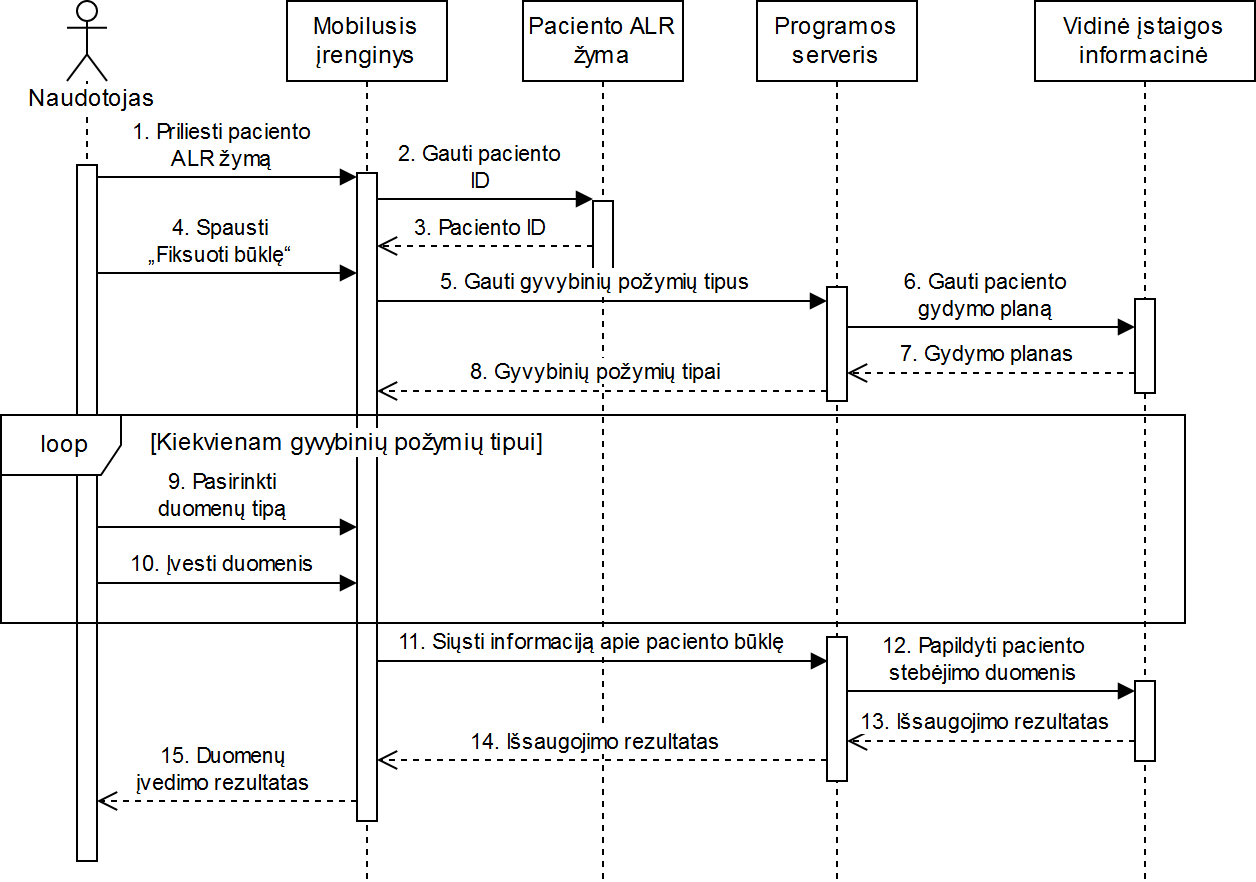
\includegraphics[scale=0.27]{images/buklesFiksavimas}
    \caption{Paciento būklės fiksavimas sekų diagrama} 
\end{figure}

Pateikta paciento būklės fiksavimo diagrama nurodo žingsnius, reikalingus užfiksuoti gautus būklės duomenis, tačiau žingsnių kiekis gali būti mažesnis, todėl toliau aptariamos šios sekų diagramos žingsnių alternatyvos.

\textbf{Paciento gydymo plano informaciją laikyti ALR žymoje}. Ši alternatyva taip pat minima medikamentų išdavimo žingsnių alternatyvose (žiūrėti 4.2.4. poskyrį), todėl argumentai, kodėl ši alternatyva nėra pasirinkta, išlieka tie patys.

\textbf{Atsisakyti gyvybinio požymio tipo pasirinkimo}. Atsisakius šio žingsnio, naudotojui nereiktų patikslinti kokie duomenys yra įvesti, t.y. ar įvesti kūno temperatūros rodikliai, ar kraujo ritmo ir t.t. Naudotojui pakaktų įvesti tinkamo formato duomenis, o sistema pagal duomenų formatą, juos validuotų ir priskirtų jiems gyvybinio požymio tipą. Pasirinkus šią alternatyvą, pirminiam agentui sumažėtų žingsnių kiekis, tačiau padidėtų duomenų formato klaidų tikimybė. Jeigu naudotojas įveda paciento kūno temperatūros duomenis širdies ritmo rodiklio formatu, sistema supranta, kad įvesti širdies ritmo duomenys, o ne kūno temperatūros.

\subsubsection{Informacinis vaizdas}
Informacinio vaizdo pateikimui naudojama esybių - ryšių diagrama, kuri nusako esybes ir ryšius tarp jų. Informacinis vaizdas yra pateiktas žemiau (žiūrėti 6 pav.), esybių aprašymas yra pateiktas lentelėje (žiūrėti 5 lentelę).

\begin{figure}[H]
    \centering
    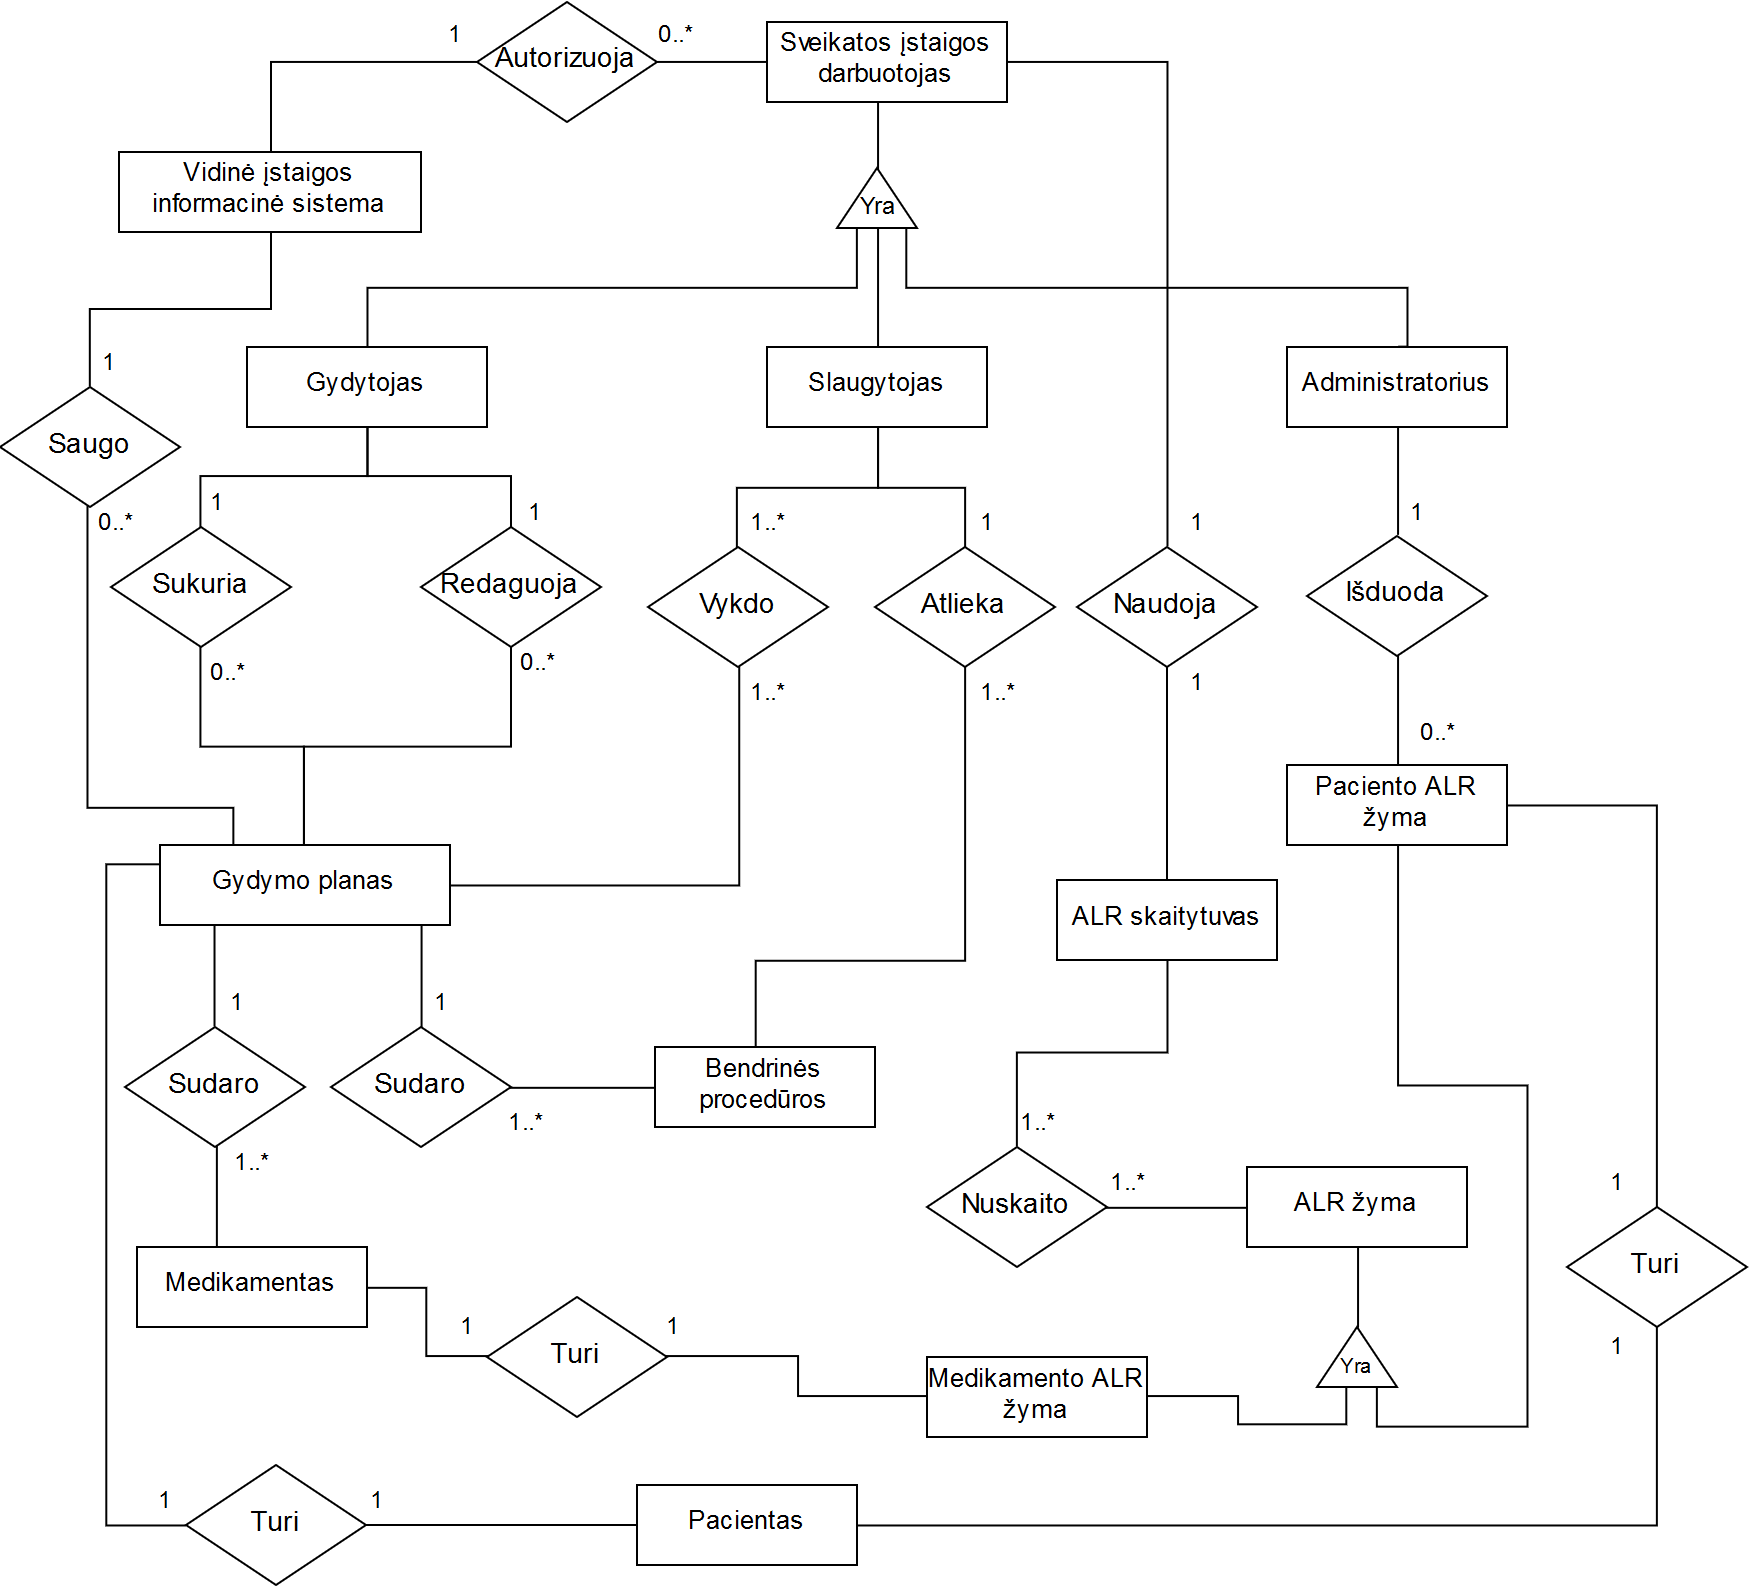
\includegraphics[scale=0.27]{images/erDiagrama}
    \caption{Esybių ryšių diagrama}
\end{figure}

\begin{table}[!ht]
    \centering
    \renewcommand{\arraystretch}{1.2}
    \renewcommand\thetable{7}

    \begin{tabular}{|m{3em}|m{12em}|m{22em}|}
    \hline 
    \rowcolor[HTML]{EFEFEF} 
    Nr. & Esybė & Aprašymas \\ \hline

    1  &  Sveikatos įstaigos darbuotojas  & Abstrakti klasė, kuri apibūdina įstaigos darbuotojus.      \\ \hline
    2  &  Gydytojas  & Informacija apie sveikatos įstaigos darbuotojas, kuris yra kvalifikuotas paskirti gydymą.     \\ \hline
    3  &  Slaugytojas  & Informacija apie sveikatos įstaigos darbuotojas, kuris prižiūri pacientus ir padeda juos gydyti.    \\ \hline
    % 4  &  Administratorius  & Informacija apie sveikatos įstaigos darbuotojas, kuris administruoja ALR žymų išdavimą.       \\ \hline
    % 5  &  Vidinė įstaigos informacinė sistema  & Vidinė įstaigos informacinė sistema, kuri autorizuoja sistemos naudotojus ir saugo duomenis \\ \hline
    % 6  &  Gydymo planas  & Informacija apie paskirtą gydymą. Gydymo plane nurodomos reikalingos procedūros, reikalingi medikamentai ir tyrimai.       \\ \hline
    % 7  &  Medikamentas  & Informacija apie medikamentą.       \\ \hline
    % 8  &  Bendrinė procedūra  & Informacija apie stacionaraus gydymo bendrinę procedūrą.       \\ \hline
    % 9  &  Pacientas  & Klinikiniai paciento duomenys.       \\ \hline
    % 10  &  ALR žyma  & Abstrakti klasė, kuri apibūdina naudojamas ALR žymas.    \\ \hline
    % 11  &  Paciento ALR žyma  & Informacija apie paciento ALR žymą, joje saugomas paciento indentifikacijos numeris.    \\ \hline
    % 12  &  Medikamento ALR žyma  & Informacija apie paciento ALR žymą, joje saugomas paciento indentifikacijos numeris, galiojimo pabaigos data.    \\ \hline
    % 13  &  ALR skaitytuvas  & Informacija apie stacionariame gydyme naudojamą ALR skaitytuvą. \\ \hlin

    \end{tabular}
    \caption{Esybių aprašymas} 

\end{table}

\begin{table}[ht!]
    \centering
    \renewcommand{\arraystretch}{1.2}
    \renewcommand\thetable{7}

    \begin{tabular}{|m{3em}|m{12em}|m{22em}|}
    \hline 
    \rowcolor[HTML]{EFEFEF} 
    Nr. & Esybė & Aprašymas \\ \hline

    % 1  &  Sveikatos įstaigos darbuotojas  & Abstrakti klasė, kuri apibūdina įstaigos darbuotojus.      \\ \hline
    % 2  &  Gydytojas  & Informacija apie sveikatos įstaigos darbuotojas, kuris yra kvalifikuotas paskirti gydymą.     \\ \hline
    % 3  &  Slaugytojas  & Informacija apie sveikatos įstaigos darbuotojas, kuris prižiūri pacientus ir padeda juos gydyti.    \\ \hline
    4  &  Administratorius  & Informacija apie sveikatos įstaigos darbuotojas, kuris administruoja ALR žymų išdavimą.       \\ \hline
    5  &  Vidinė įstaigos informacinė sistema  & Vidinė įstaigos informacinė sistema, kuri autorizuoja sistemos naudotojus ir saugo duomenis \\ \hline
    6  &  Gydymo planas  & Informacija apie paskirtą gydymą. Gydymo plane nurodomos reikalingos procedūros, reikalingi medikamentai ir tyrimai.       \\ \hline
    7  &  Medikamentas  & Informacija apie medikamentą.       \\ \hline
    8  &  Bendrinė procedūra  & Informacija apie stacionaraus gydymo bendrinę procedūrą.       \\ \hline
    9  &  Pacientas  & Klinikiniai paciento duomenys.       \\ \hline
    10  &  ALR žyma  & Abstrakti klasė, kuri apibūdina naudojamas ALR žymas.    \\ \hline
    11  &  Paciento ALR žyma  & Informacija apie paciento ALR žymą, joje saugomas paciento identifikacijos numeris.    \\ \hline
    12  &  Medikamento ALR žyma  & Informacija apie paciento ALR žymą, joje saugomas paciento identifikacijos numeris, galiojimo pabaigos data.    \\ \hline
    13  &  ALR skaitytuvas  & Informacija apie stacionariame gydyme naudojamą ALR skaitytuvą. \\ \hline


    \end{tabular}
    \caption{Esybių aprašymas} 

\end{table}

\subsection{Projektuojamos sistemos prototipas}
Šiame poskyryje yra aprašomas projektuojamos sitemos prototipas. Prototipo tikslas - išsiaiskinti ar pagrindinius sistemos scenarijus įmanoma įgyvendinti. Šiame poskyryje pirmiausiai aprašomi prototipo uždaviniai, po to aprašoma realizacija ir prototipo testavimas.

\subsubsection{Uždaviniai}
Prototipo tikslui pasiekti išsikelti šie uždaviniai:

\begin{itemize}
    \item Nuskaityti paciento ALR žymą;
    \item Nuskaityti medikamento ALR žymą;
    \item Gauti paciento gydymo planą;
    \item Užfiksuoti paciento būklę;
    \item Verifikuoti medikamento išdavimą.
\end{itemize}

\subsubsection{Realizacija}
Prototipo įgyvendinimui buvo pasirinkti „React Native“ ir „Express.js“ karkasai. „React Native“ skirtas kurti mobiliąsias aplikacijas. Šis karkasas pasirinktas dėl to, kad parašius aplikacijos kodą „Javascript“ programavimo kalba, karkasas pasirūpina, kad aplikacija veiktų tiek „iOS“, tiek „Android“ operacinėse aplinkose, todėl nereikia kurti dviejų atskirų aplikacijų, kurios būtų pritaikytos šioms dviems operacinėms sistemoms. „Express.js“ skirtas kurti vidinę sistemos dalį. Šis karkasas buvo pasirinktas dėl to, kad programinis kodas yra rašomas su „Javascript“ programavimo kalba, todėl sistemos tiek išorinė, tiek vidinė dalis yra rašoma ta pačia programavimo kalba. Šis karkasas taip pat leidžia greitai kurti vidinę sistemos dalį, o kadangi kuriamas sistemos prototipas, „Express.js“ tinka išsikeltiem uždaviniam atlikti.


Pirmiausiai buvo kuriama vidinė sistemos dalis. Kadangi siūloma, jog duomenų saugojimas būtų vykdomas sveikatos įstaigų vidinių sistemų pagalba, duomenų saugojimui nebuvo kuriama duomenų bazė, o duomenys saugomi failinėje sistemoje. Vidinėje sistemos dalyje buvo sukurti 4 galutiniai taškai (angl. \textit{endpoint}), kurie priima mobiliosios aplikacijos užklausas ir grąžina atsakymą. Šie galutiniai taškai atlieka šiuos funkcionalumus: 
\begin{itemize}
    \item Patikrina ar išduodamas tinkamas medikamentas;
    \item Grąžina pacientui aktualius gyvybinių požymių tipus;
    \item Priima ir išsaugo informaciją apie paciento būklę;
    \item Grąžina visą informaciją, kuri susijusi su pacientu. Šį funkcionalumą atliekantis galutinis taškas yra naudojamas testuojant sistemos veikimą;
\end{itemize}
Sukūrus vidinę sistemos dalį, buvo kuriama mobilioji aplikacija. Tam, kad aplikacija galėtų pasiekti nuskaitytus ALR žymos duomenis, buvo pasirinkta naudoti „react-native-nfc-manager“ biblioteką,  kuri palengvina darbą su ALR technologija. Nuskaičius ALR žymą ir gavus joje esančius duomenis, aplikacija iškoduoja gautus duomenis. Turint paciento ID, pagal naudotojo pasirinkimą, aplikacija arba laukė kol nuskaitys medikamento ALR žymą, arba gavus pacientui aktualius gyvybinių požymių tipus, laukė kol vartotojas suves informaciją apie paciento būklę (žiūrėti 7 pav., 8 pav., 9 pav., 11pav. ). Turint visą reikiamą informaciją, aplikaciją kreipėsi į vidinę sistemos dalį. Prototipo reealizacija leidžia keliems naudotojams naudotis sistema (žiūrėti 10 pav., 12 pav.).



\subsubsection{Testavimas}

Sukūrus prototipą, testavimas buvo atliekamas 3 etapais:
\begin{enumerate}
    \item Mobiliosios aplikacijos funkcionalumo testavimas;
    \item Vidinės sistemos dalies funkcionalumo testavimas;
    \item Pagrindinius sistemos scenarijų testavimas;
\end{enumerate}

Sistemos prototipo testavimo metu buvo naudojami šie įrenginiai:
\begin{itemize}
    \item Mobilusis įrenginys Nokia 6.1 su Android 9 operacine sistema;
    \item Mobilusis įrenginys Samsung Galaxy S6 su Android 7 operacine sistema;
    \item Mobilusis įrenginys Iphone 8 su iOS 11 operacine sistema;
    \item 4 NXP MIFARE Ultralight C ALR žymos, kurios paremtos ISO 14443-3A standartu;
\end{itemize}

Testuojant mobiliąja aplikaciją, pirmiausiai buvo testuojamas ALR žymų nuskaitomumas. Visi 3 mobilieji įrenginiai sugebėjo nuskaityti duomenis esančius ALR žymoje. Ištestavus ALR nuskaitomumą, pradėta testuoti tinkamų vaizdų parodymas aplikacijoje ir komunikavimas su vidine sistemos dalimi. Nors mobiliajame įrenginyje, kuris turi iOS operacinę sistemą, mobiliosios aplikacijos vaizdai nežymiai skyrėsi nuo Android įrenginių, tačiau tai neturėjo įtakos mobiliosios aplikacijos funkcionalumui.

Testuojant vidinės sistemos dalies funkcionalumą, buvo naudojamas „Postman“ įrankis. Kadangi vidinės sistemos dalies pagrindinis funkcionalumas - priimti, verifikuoti iš išsaugoti duomenis, buvo pakartotinai siuntinėjamos įvairios užklausos su tinkamais ir netinkamais duomenimis.

Pagrindinių sistemos scenarijų testavimo metu, su skirtingais įrenginiais buvo atliekami 4 skyriuje aprašyti scenarijai. Primiausiai su „NFC tool“ įrankiu buvo paruošiamos 2 paciento ALR žymos ir 2 medikamento ALR žymos. Su visais 3 mobiliais įrenginiais buvo tikrinamas medikamentų verifikavimas ir pacientų būklės fiksavimas. Atlikus testavimus paaiškėjo, jog pagrindinius sistemos scenarijus įmanoma įgyvendinti, todėl išsikeltas prototipo tikslas buvo pasiektas.

\sectionnonum{Rezultatai ir išvados}
Šiame darbe išanalizuota stacionaraus gydymo situacija lietuvoje, identifikuotos problemos, o kartu ir apžvelgiami šių problemų sprendimo būdai. Taip pat darbe aprašytos ir išnagrinėtos sveikatos priežiūros įstaigų informacinės sistemos. Nagrinėjant artimojo lauko ryšio technologiją, išsiaiškinta, kad ši technologija yra tinkama stacionariame gydyme teikiamų paslaugų efektyvimo didinimui. Šiame dare yra siūloma artimojo lauko ryšio technologija pagrįstas programų sistemų architektūra ir pateikiamos jos prototipas

Atlikus darbą buvo gauti šie \textbf{rezultatai}:
\begin{enumerate}
    \item Nustatyta kas yra stacionarus gydymas, kokia jo situacija Lietuvoje ir identifikuotos stacionariame gydyme kylančios problemos bei nustatyti šių problemų sprendimo būdai;
    \item Aliktas Lietuvos sveiktos priežiūros įstaigų informacinių sistemų palyginimas, išanalizuota elektroninės sveikatos paslaugų ir bendradarbiavimo infrastruktūros informacinė sistema ir nustatyti integraciniai reikalavimai;
    \item Remiantis literatūra, išanalizuotas ALR technologijos veikimas, nustatytos pritaikymo galimybės sveikatos priežiūroje;
    \item Iškelti programų sistemų architektūros funkciniai ir nefunkciniai reikalavimai, analizės būdų nustatyti ir pasiūlyta architektūra, sukurtas sistemos prototipas.
\end{enumerate}

Darbo \textbf{išvados}:
\begin{enumerate}
    \item Stacionariame gydyme teikiamų paslaugų efektyvumas nėra aukštas, tačiau ALR technologija gali prisidėti prie sėkmingo aplinkos intelekto įgyvendinimo sveikatos priežiūros sektoriuje ir didinti stacionariame gydyme teikiamų paslaugų efektyvumą;
    \item Ne visos sveikatos priežiūros įstaigos turi vidines informacines sistemas, tačiau įstaigų, turinčių šias sistemas, informacinės sistemos nėra vienodos, jų sudėtingumo lygiai ir teikiami funkcionalumai skiriasi. Informacinių sistemų sudėtingumas priklauso nuo įstaigos dydžio;
    \item Norint įdiegti naują technologiją į sveikatos priežiūros sektorių, dėl įstaigų informacinių sistemų nevienodumo, verta kurti atskirą informacinę sistemą ir atlikti integraciją su esamomis informacinėmis sistemomis;
    \item Sveikatos priežiūros įstaigų naudojamas informacines sistemas yra svarbu kurti taip, jog jos būtų paprastos naudojimui, nesudėtingai plečiamos ir užtikrintų pacientų duomenų saugumą;
    \item Siūlomos sistemos įgyvendinimo kaštai kiekvienai sveikatos priežiūros įstagai skiriasi. Tai priklauso nuo to, ar įstaiga turi savo vidinę informacinę sistemą, kuri yra integruota į elektroninės sveikatos paslaugų ir bendradarbiavimo infrastruktūros informacinę sistemą, ar tokios sistemos neturi.
    \item Įgyvendinus ir atliktus siūlomos sistemos prototipo testavimą, galima teigti, kad siūloma ALR technologija paremta sistema, kuri padeda atlikti efektyviau bendrines stacionaraus gydymo procedūras, yra įgyvendinama.
\end{enumerate}

Viską apibendrinus galima teigti, kad išsikeltas darbo tikslas buvo pasiektas. Išnagrinėta Lietuvos stacionaraus gydymo situacija, identifikuotos problemos, apželgti šių problemų sprendimo būdai ir analizuojant alternatyvas, pasiūlytas programų sistemų architektūros sprendimas, kuris didina stacionaraus gydymo efektyvumą.

Ateityje šį darbą galima tęsti šiais aspektais:
\begin{enumerate}
    \item Sukurti pilnai veikiantį siūlomos programų sistemos architektūros sprendimą ir integruoti į pasirinktą sveikatos priežiūros įstaigą;
    \item Išanalizuoti ir atlikti žmogaus gyvybinių požymių sensorių diegimą į siūlomą sistemą;
\end{enumerate}

\printbibliography[heading=bibintoc]  


\appendix 
\section{Prototipas}

\begin{figure}[H]
    \centering
    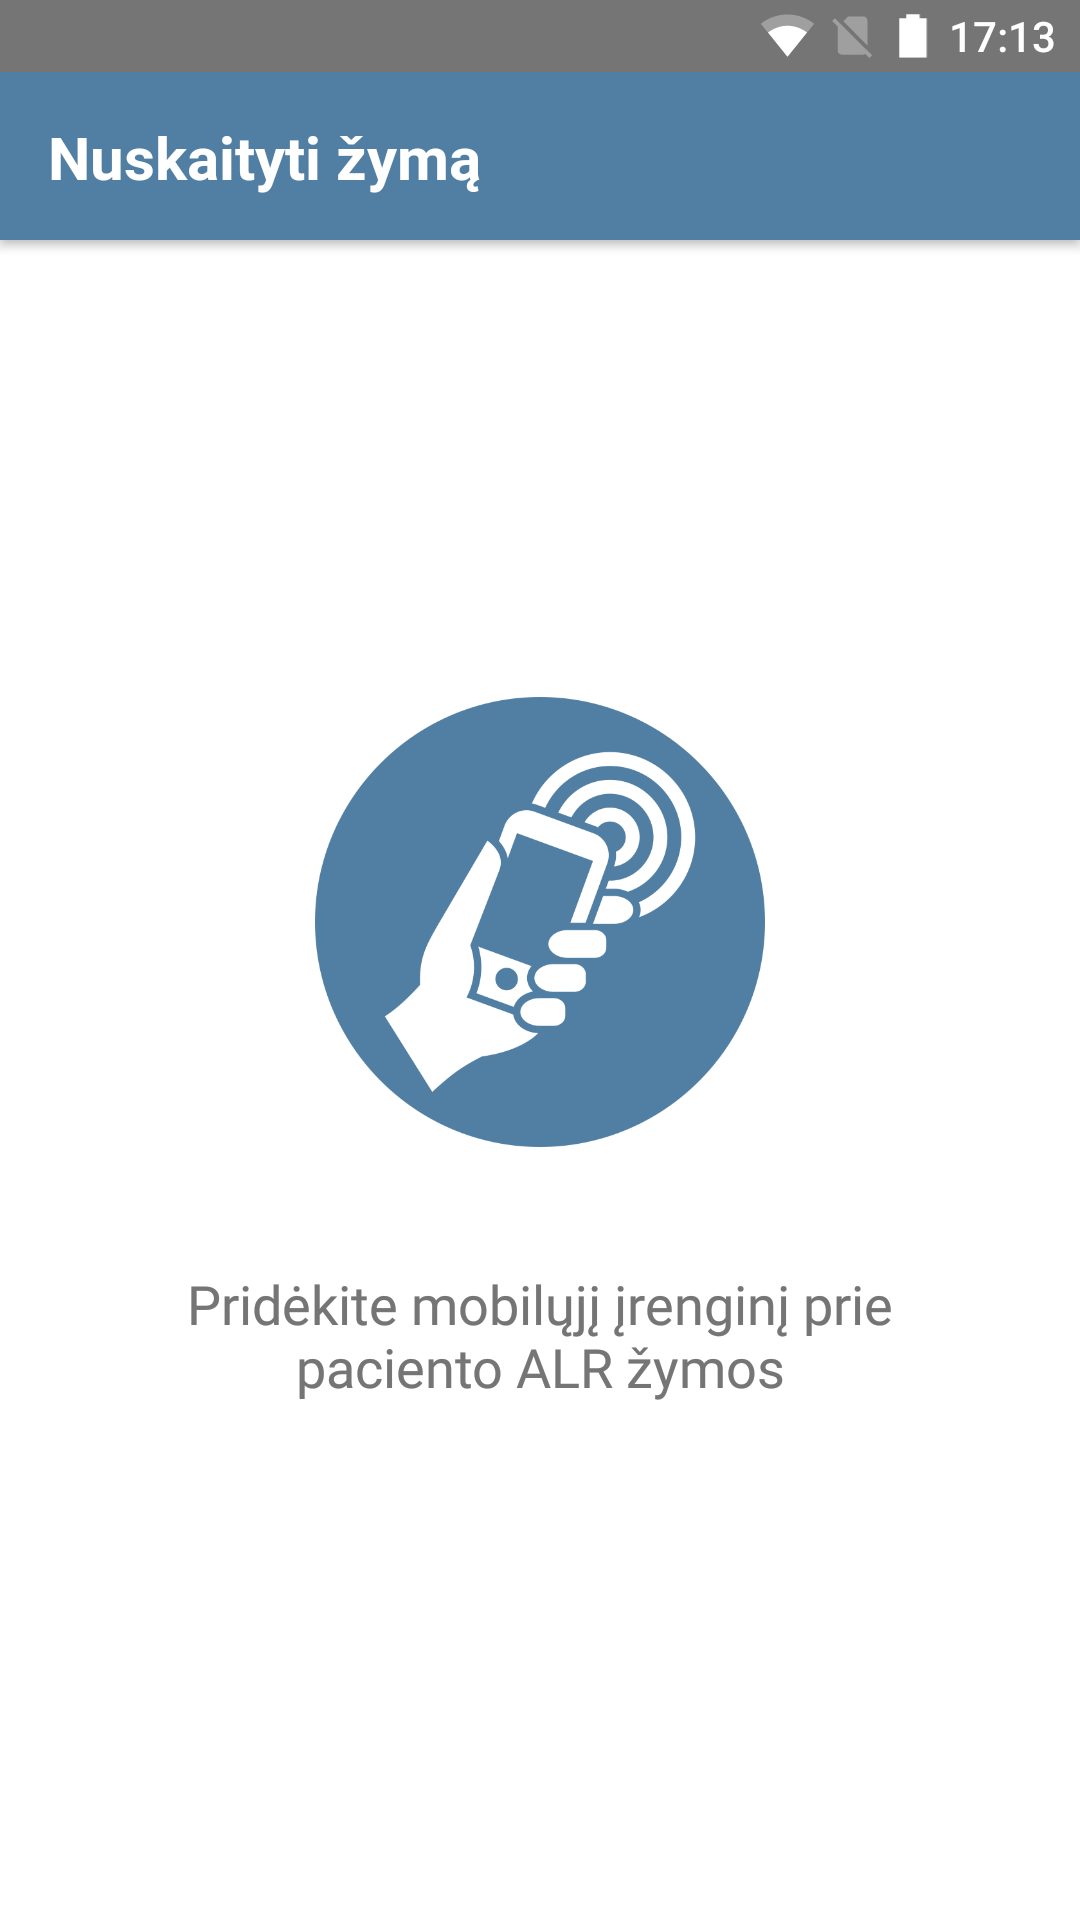
\includegraphics[scale=0.15]{images/prototype-3}
    \caption{Laukiama kol naudotojas priliest paciento ALR žymą} 
\end{figure}

\begin{figure}[H]
    \centering
    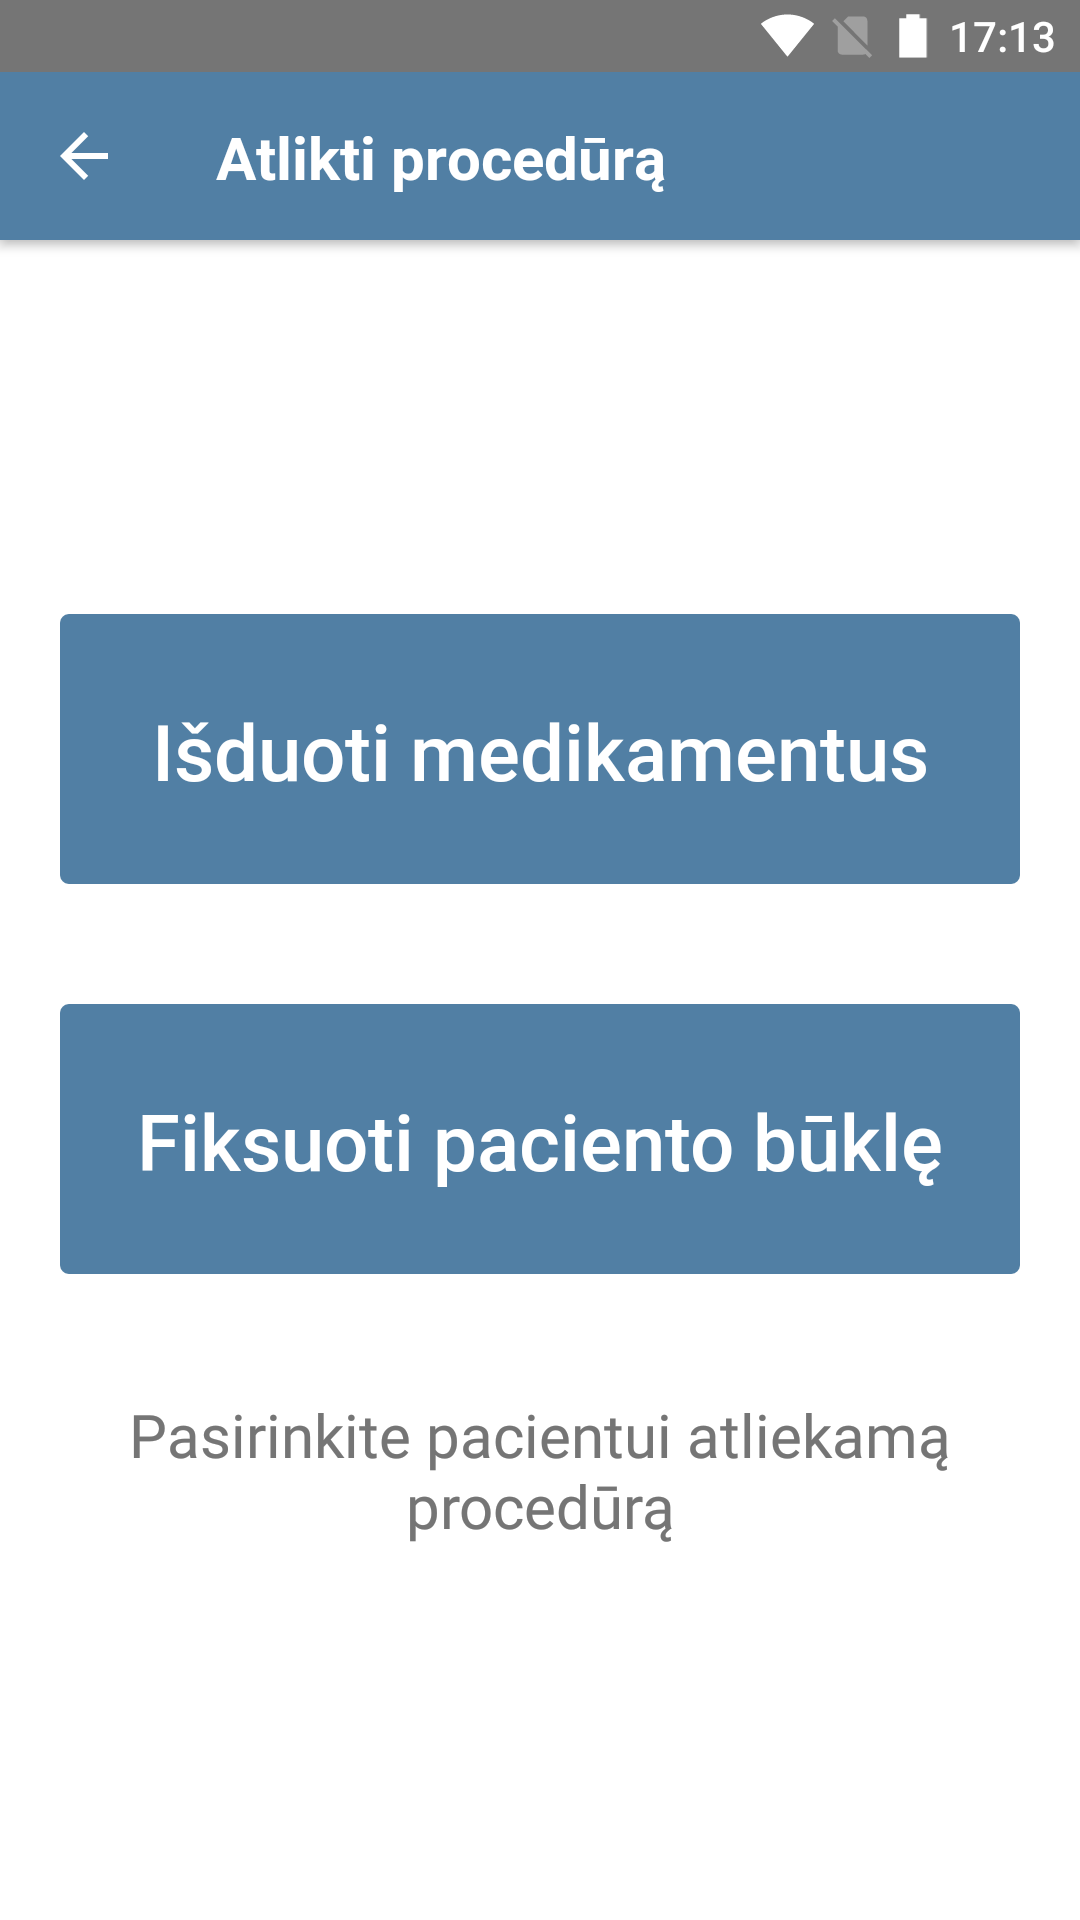
\includegraphics[scale=0.15]{images/prototype-5}
    \caption{Atliekamų procedūrų pasirinkimas} 
\end{figure}

\begin{figure}[H]
    \centering
    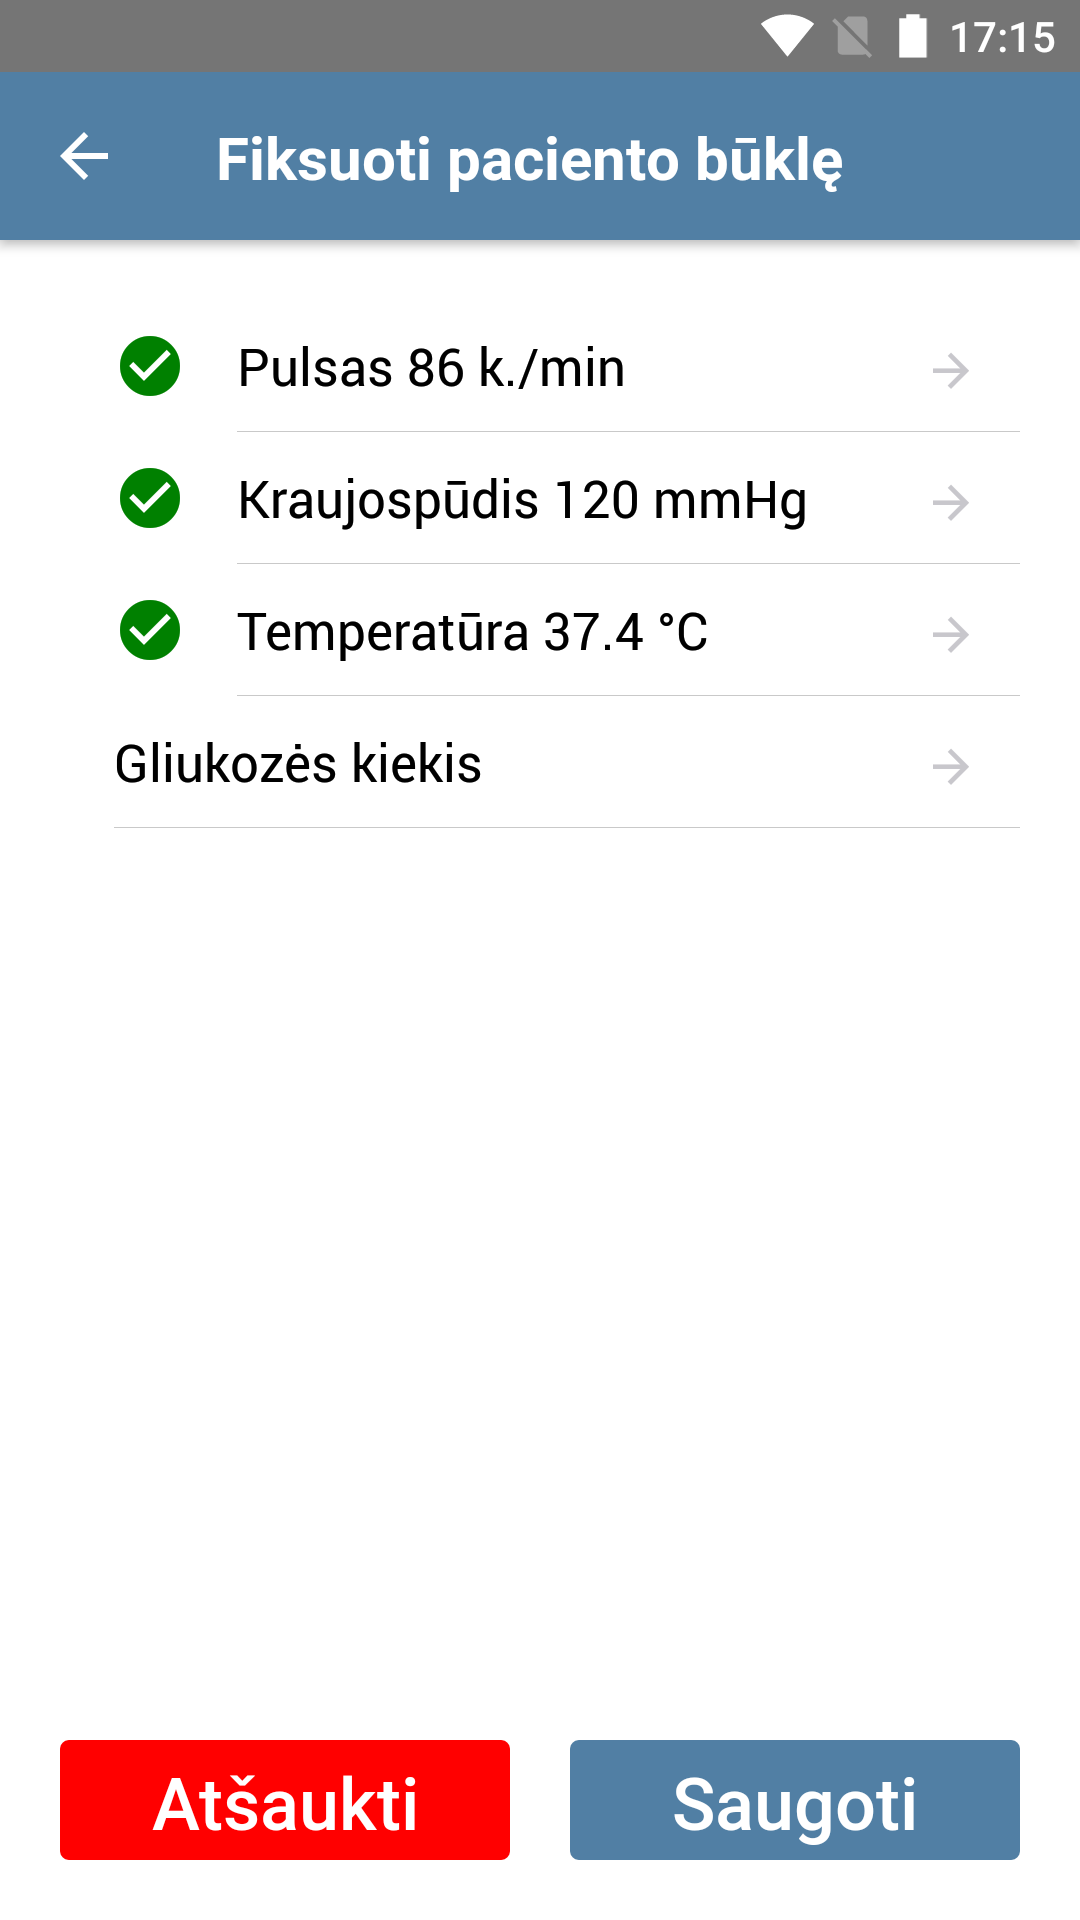
\includegraphics[scale=0.15]{images/prototype-6}
    \caption{Paciento būklės fiksavimas} 
\end{figure}

\begin{figure}[H]
    \centering
    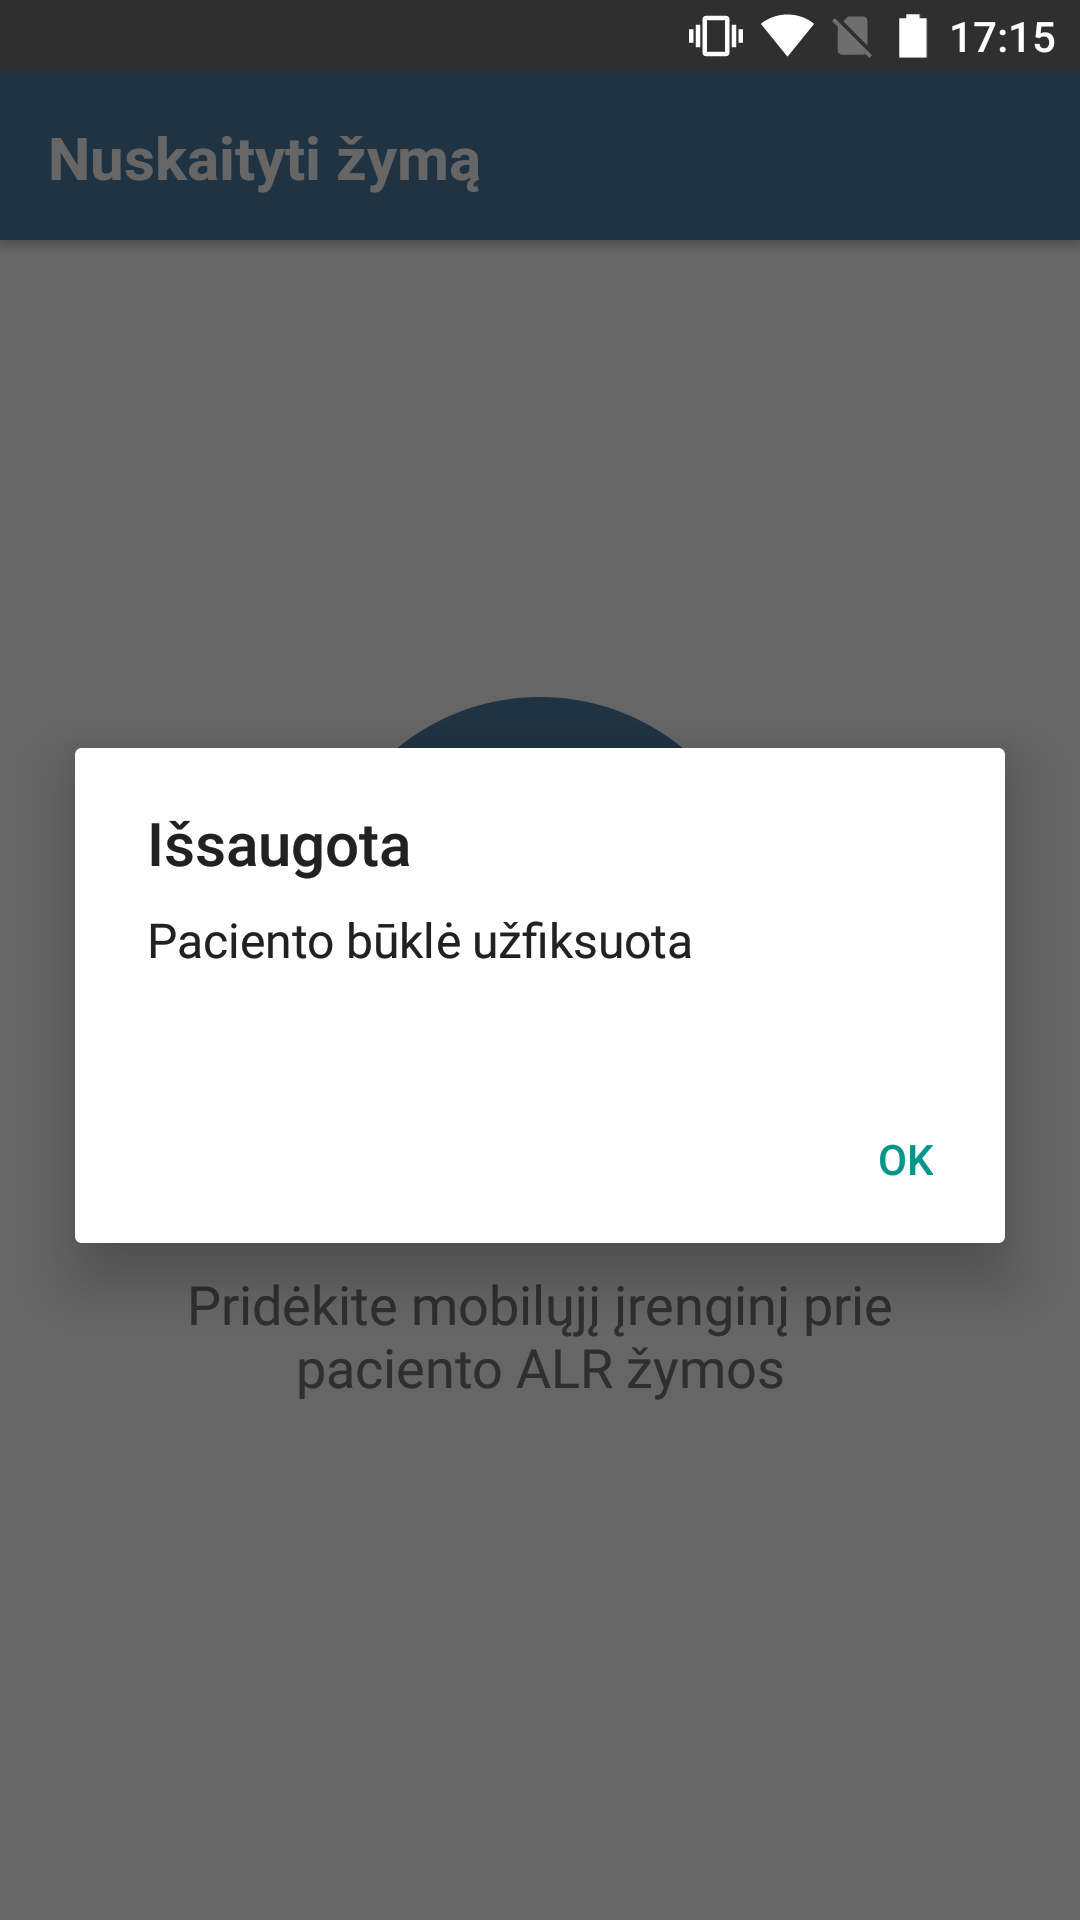
\includegraphics[scale=0.15]{images/prototype-1}
    \caption{Paciento būklės fiksavimo patvirtinimas} 
\end{figure}

\begin{figure}[H]
    \centering
    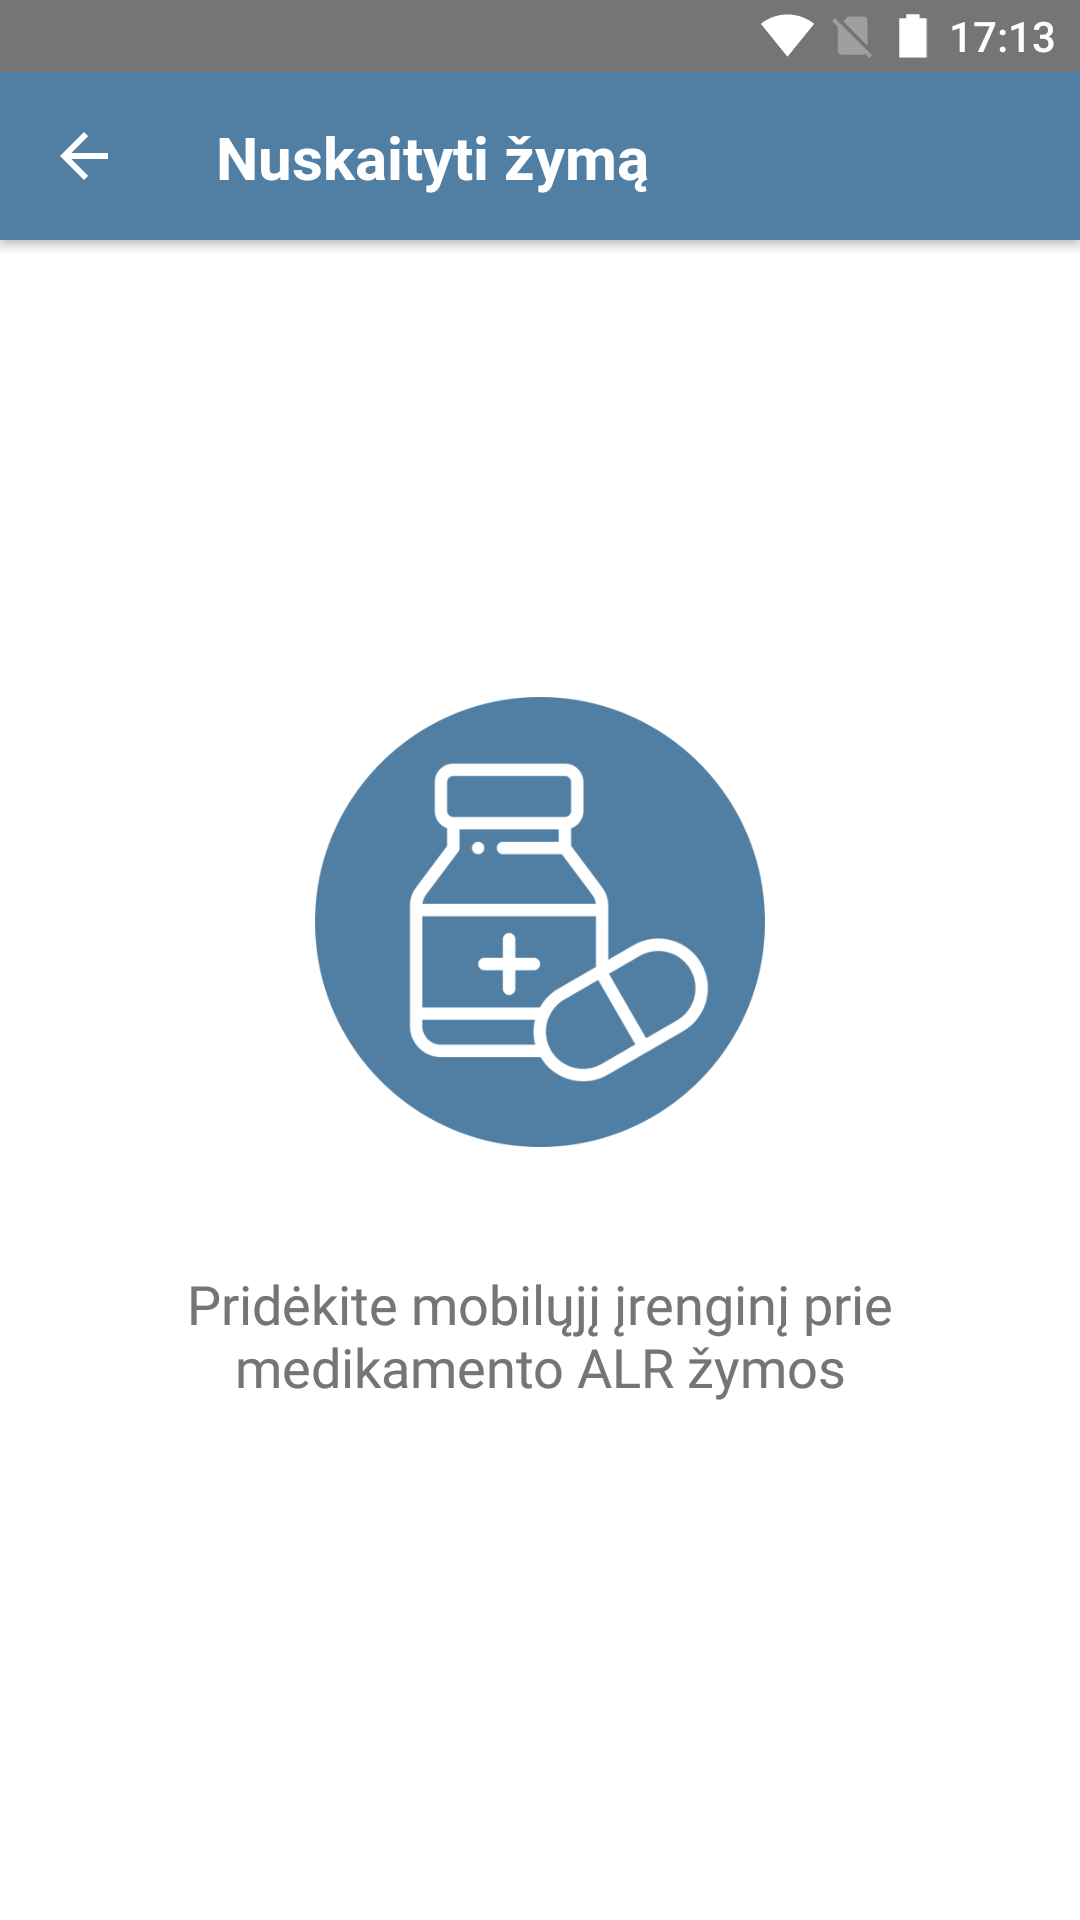
\includegraphics[scale=0.15]{images/prototype-2}
    \caption{Laukiama kol naudotojas prilies medikamento ALR žymą} 
\end{figure}

\begin{figure}[H]
    \centering
    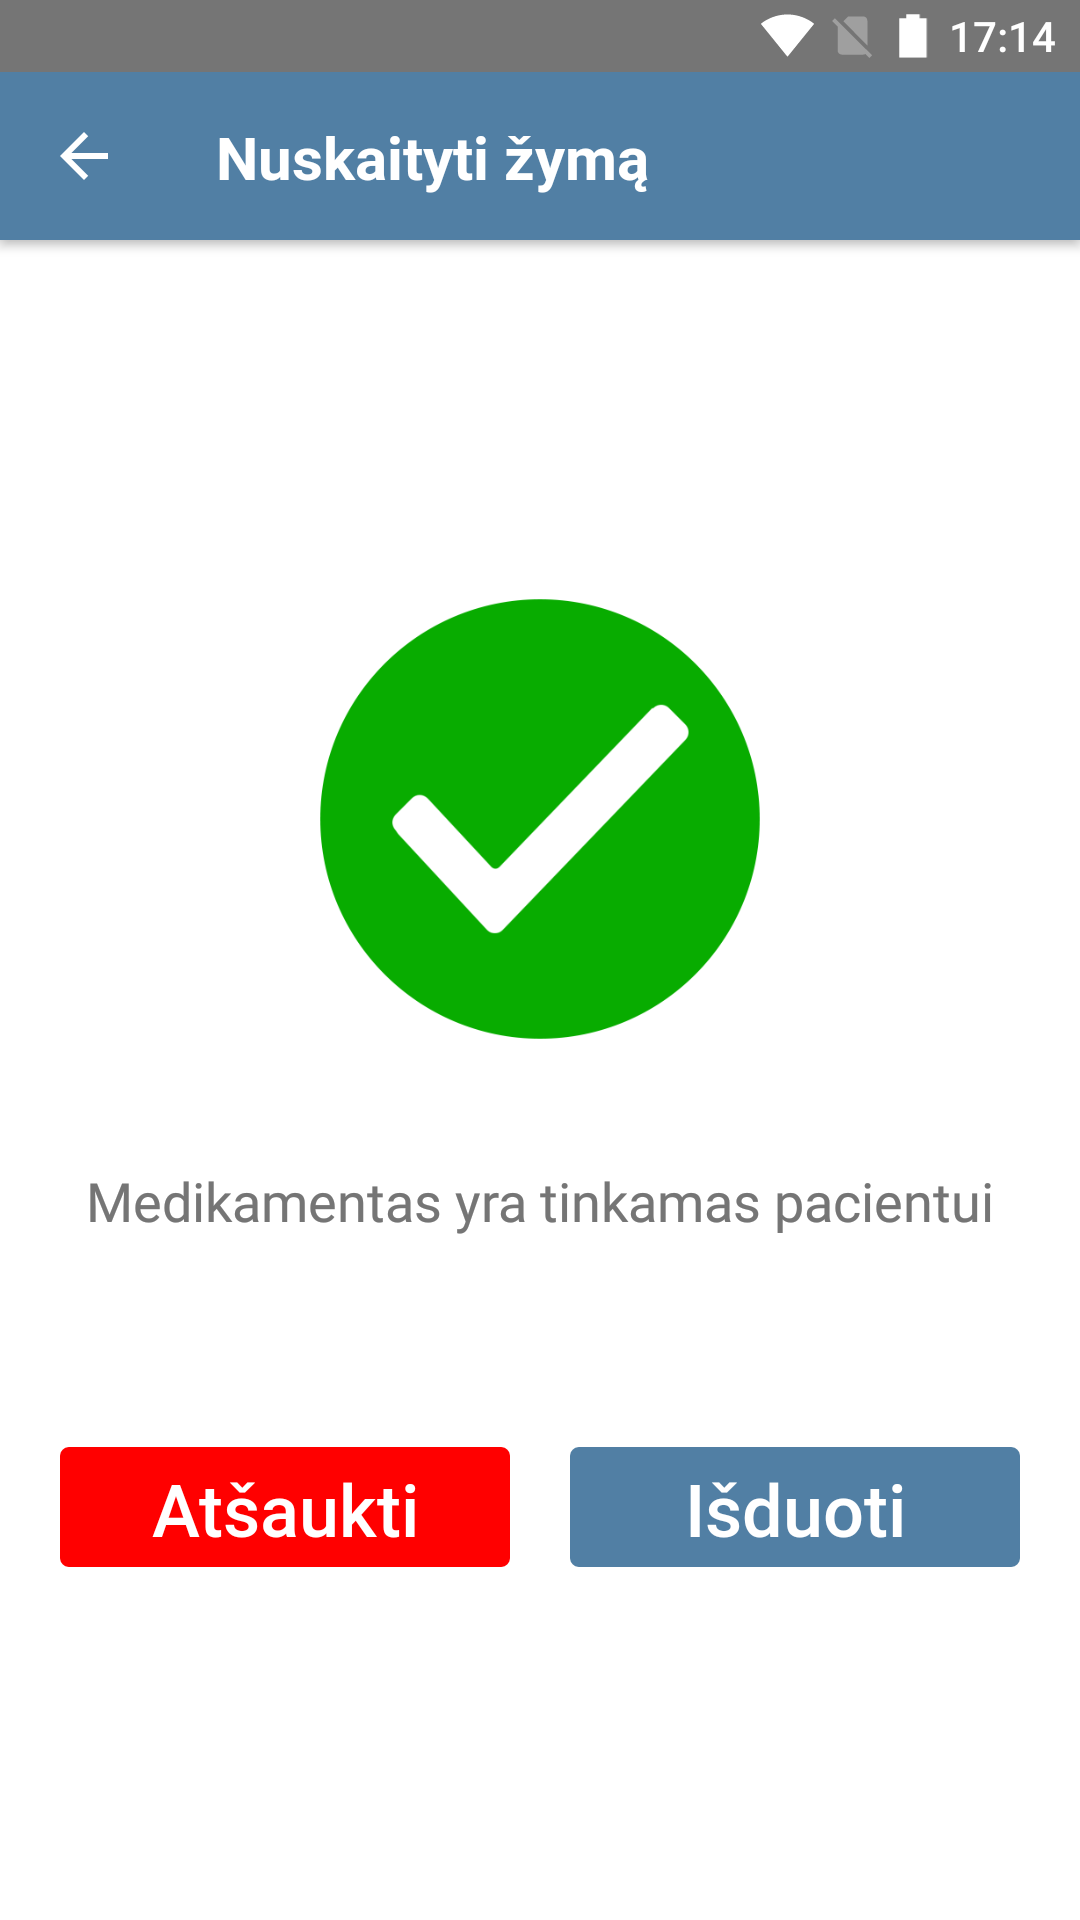
\includegraphics[scale=0.15]{images/prototype-4}
    \caption{Medikamento verifikavimo rezultatas} 
\end{figure}

\end{document}
